\section{Thiết kế}


\subsection{Thiết kế tổng thể}


\subsubsection{Kiến trúc tổng thể}
Hệ thống \texttt{YOLOHome} được thiết kế và xây dựng như một giải pháp giám sát và điều khiển nhà thông minh hoàn chỉnh, kết hợp hài hòa giữa các tầng công nghệ từ phần cứng đến phần mềm. Kiến trúc hệ thống bao gồm bốn thành phần cốt lõi:
\begin{itemize}
    \item \textbf{Giao diện người dùng Web SPA}: Được phát triển trên nền tảng thư viện React 19 kết hợp công cụ build Vite, chạy trên môi trường containerized phục vụ bởi Nginx. Giao diện cung cấp khả năng quan sát trực quan các thông số môi trường theo thời gian thực và cho phép bật/tắt thiết bị thủ công cùng tính năng Push-to-Talk điều khiển bằng giọng nói.
    \item \textbf{Tầng Backend REST API \& MQTT Layer}: Sử dụng framework Express 5 chạy trên nền tảng Node.js kết hợp với hệ quản trị cơ sở dữ liệu phi quan hệ MongoDB. Tầng này chịu trách nhiệm điều phối các yêu cầu REST từ client, tích hợp các bộ chuyển dịch AI, lưu trữ dữ liệu snapshot môi trường, vết điều khiển (\texttt{ControlTrace}), nhật ký cảnh báo (\texttt{Alert}), và xuất bản các lệnh tới các chủ đề (topics) trên MQTT Broker Mosquitto.
    \item \textbf{Cầu nối trung gian Gateway}: Viết bằng ngôn ngữ lập trình Python, đóng vai trò chuyển đổi giao thức hai chiều giữa mạng tin nhắn MQTT phi tập trung và Kit phần cứng Yolo:Bit kết nối vật lý qua đường truyền USB Serial với băng thông ổn định. Gateway chịu trách nhiệm bóc tách các gói tin Serial dạng rút gọn và thực thi logic tự động hóa cục bộ dựa trên ngưỡng cấu hình hoặc mô hình AI Decision Tree.
    \item \textbf{Kit phần cứng vật lý}: Sử dụng vi điều khiển Yolo:Bit kết hợp hệ cảm biến đo đạc môi trường DHT22 (đo nhiệt độ, độ ẩm), quang trở LDR/BH1750 (đo ánh sáng) cùng các thiết bị chấp hành thực tế bao gồm đèn LED chiếu sáng, Quạt thông gió động cơ DC (Fan) và Động cơ Servo điều khiển rèm cửa.
    \item \textbf{Các dịch vụ phụ trợ AI}: Bao gồm dịch vụ nhận dạng giọng nói tiếng Việt Vosk STT và mô hình phân loại ý định ML được triển khai dưới dạng microservices độc lập, giao tiếp qua REST API với tầng Backend để cung cấp khả năng điều khiển bằng giọng nói thông minh.
\end{itemize}

Dưới đây là sơ đồ kiến trúc tổng thể của hệ thống. Trong quá trình phát triển, sơ đồ này được thiết kế và mô tả bằng ngôn ngữ Mermaid để phục vụ cho việc tự động kết xuất hình ảnh.

% Mermaid Source Code cho sơ đồ kiến trúc tổng thể:
% flowchart LR
%   subgraph Browser["Browser — React SPA (Vite :5173 / Nginx :8080)"]
%     UI[Pages: Login / Dashboard / DeviceManagement]
%     VC[VoiceControl<br/>RecordRTC press-to-talk]
%   end
% 
%   subgraph BE["Node.js Backend (Express :5000)"]
%     REST[REST routes<br/>/api/users · /api/sensors<br/>/api/devices · /api/alerts<br/>/api/system · /api/voice]
%     SVC[Services<br/>SensorService · DeviceService<br/>AlertService · VoiceService]
%     MQB[MQTT layer<br/>mqttClientService · mqttService]
%   end
% 
%   subgraph AUX["Auxiliary microservices"]
%     VOSK[Vosk STT<br/>FastAPI :8500<br/>POST /transcribe]
%     ML[ML intent classifier<br/>FastAPI :8000<br/>POST /predict]
%   end
% 
%   MONGO[("MongoDB :27017<br/>Sensor · Device · Alert<br/>ThresholdTrace · ControlTrace · User")]
%   BROKER{{"Mosquitto MQTT broker :1883"}}
% 
%   subgraph GW["Python Gateway"]
%     GMQ[Bridge.MQTTClient]
%     CTRL[Controller.MainController<br/>rate-limited bus]
%     ADP[Adapter.DefaultDataAdapter<br/>JSON ⇄ !ABBR:VAL#]
%     SER[Serial.SerialModule<br/>background reader]
%     THR[ThresholdService]
%     AI[AIService<br/>DecisionTree.pkl, optional]
%   end
% 
%   KIT[("Yolo:Bit kit<br/>DHT22 · LDR/BH1750<br/>LED · Fan · Servo")]
% 
%   UI -- "HTTP/JSON · poll 5–10 s" --> REST
%   VC -- "POST audio/wav (multipart)" --> REST
%   REST --> SVC
%   SVC <--> MONGO
%   SVC --> MQB
%   REST -- "POST /transcribe" --> VOSK
%   REST -- "POST /predict" --> ML
%   MQB <-- "home/+/device/+/{set,state}<br/>home/+/sensor/+<br/>home/system/{getall,stateall}" --> BROKER
%   BROKER <--> GMQ
%   GMQ <--> CTRL
%   CTRL <--> ADP
%   ADP <-- "!ABBR:VAL#  @ 115200 baud" --> SER
%   SER <--> KIT
%   CTRL --> THR
%   CTRL --> AI
\begin{figure}[H]
    \centering
    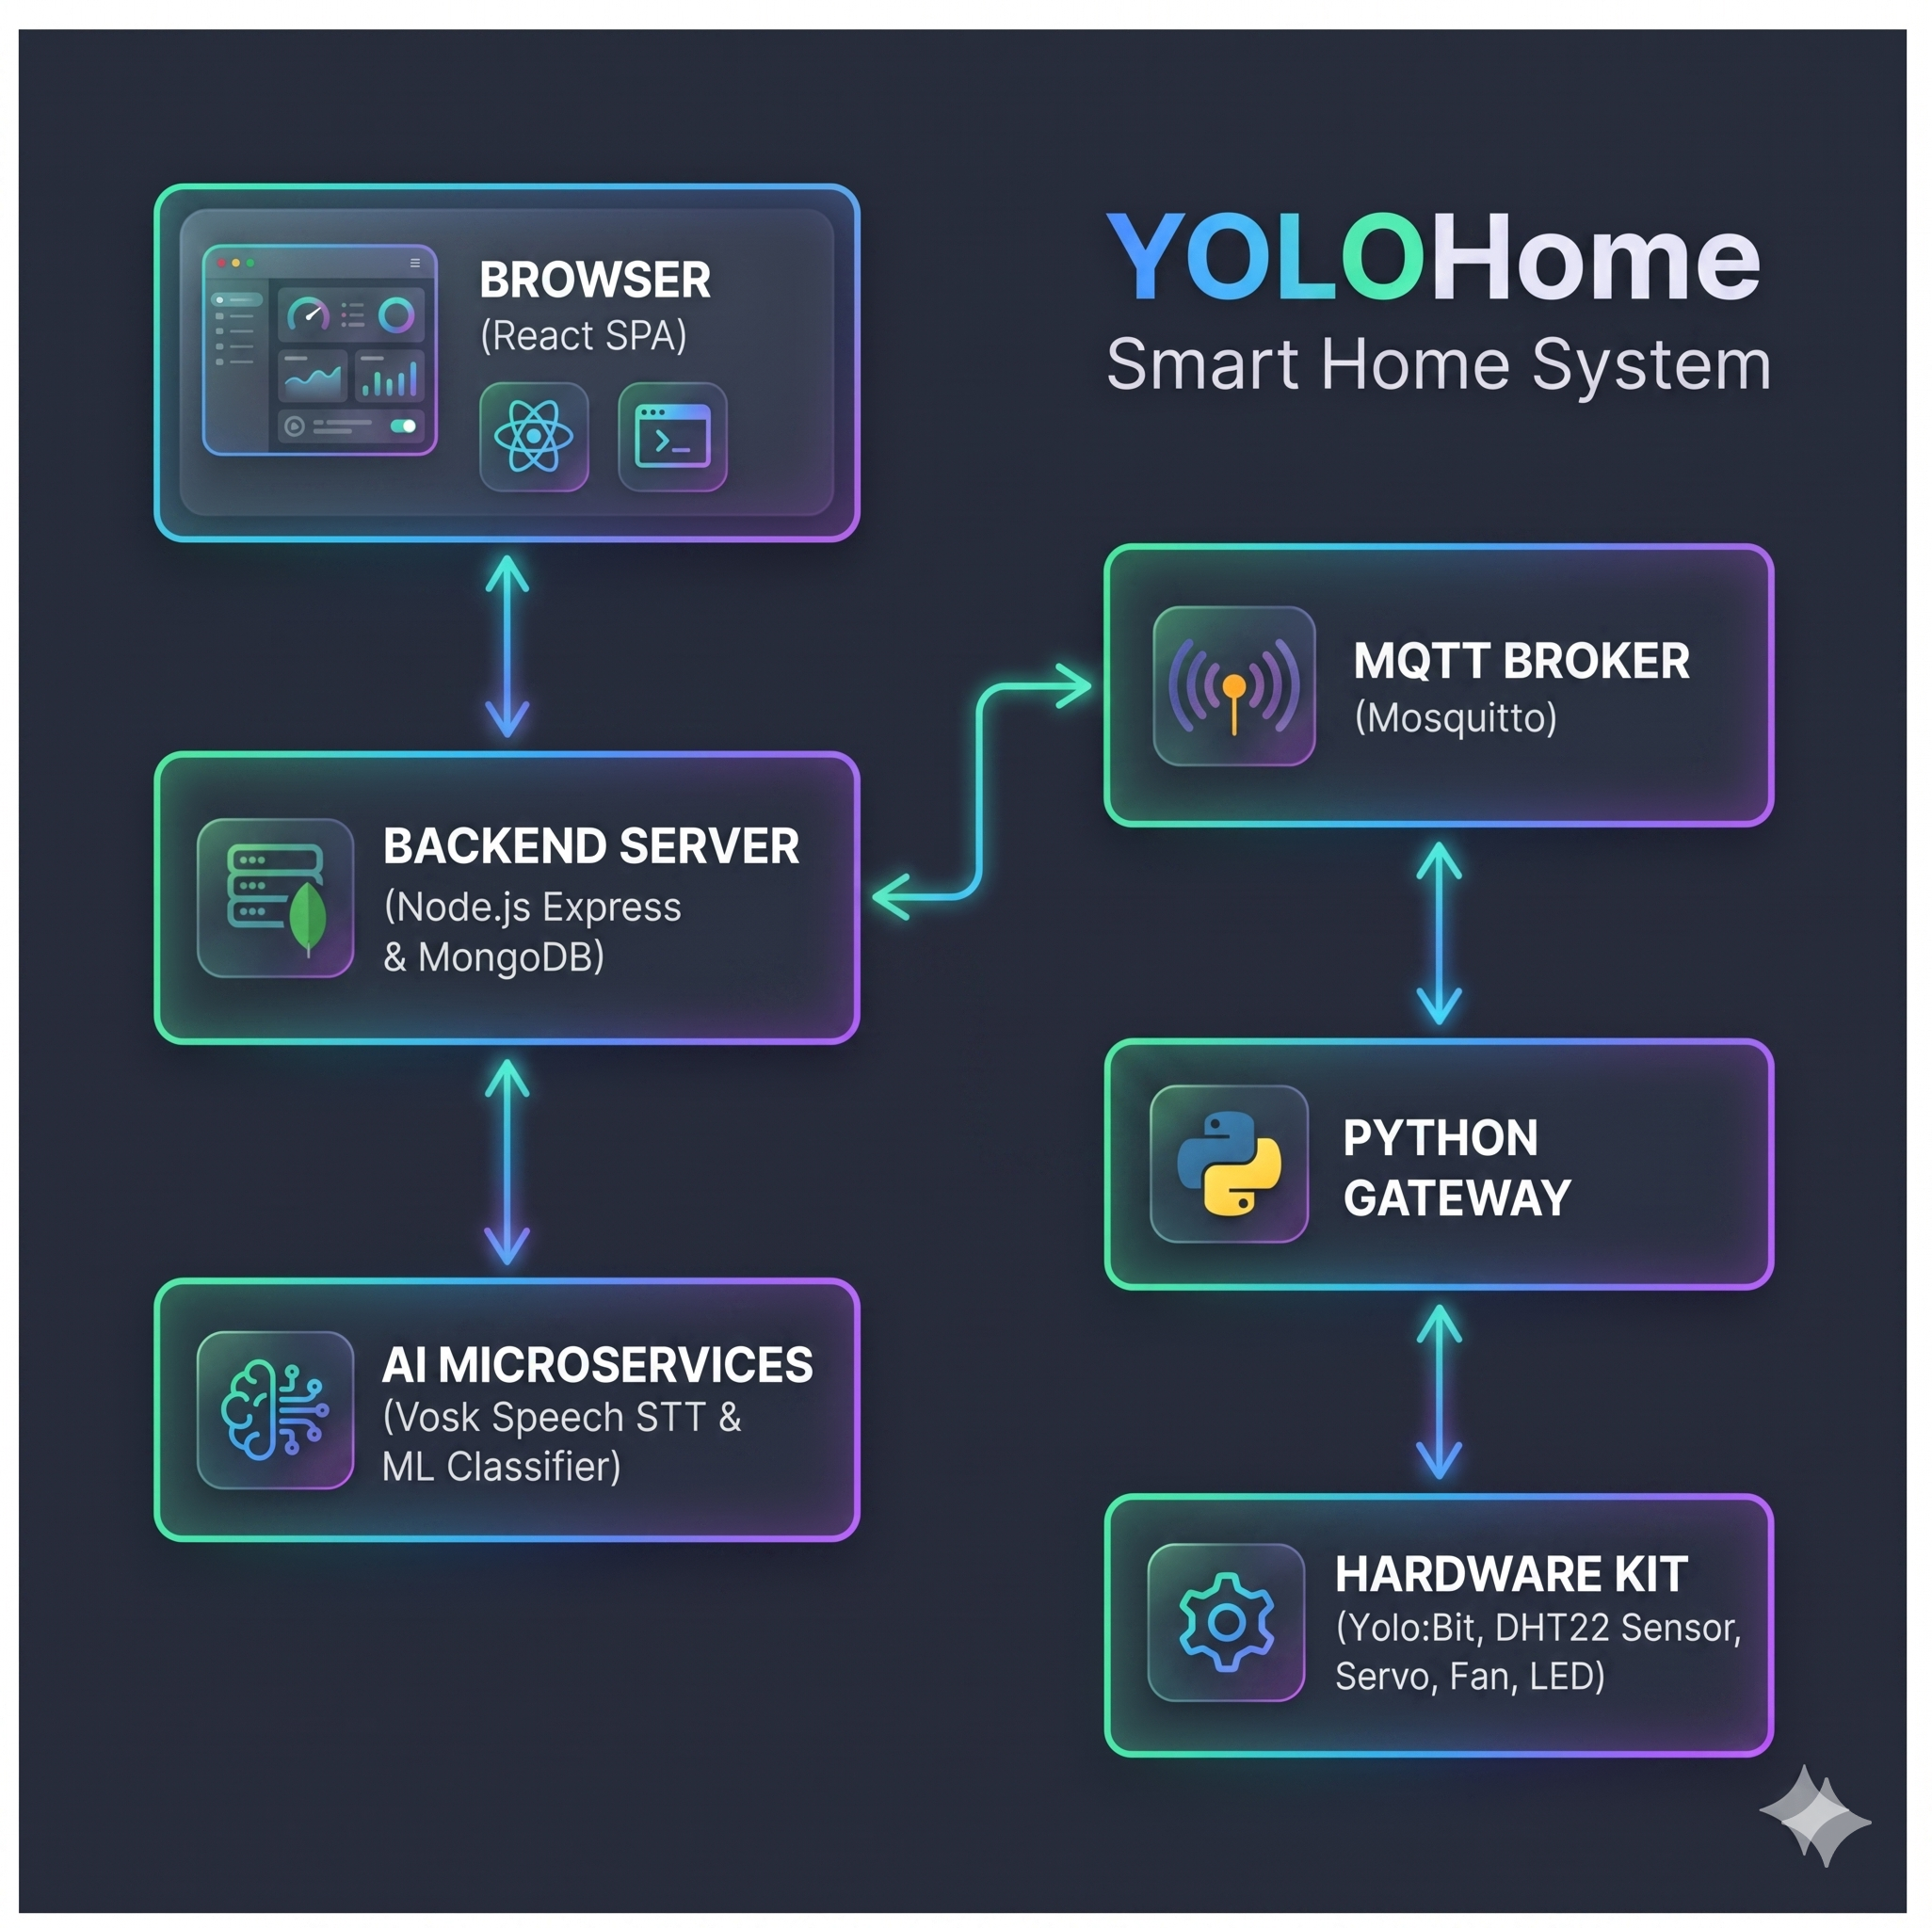
\includegraphics[width=0.95\textwidth]{figures/kien-truc-tong-the.png}
    \caption{Sơ đồ kiến trúc tổng thể hệ thống YOLOHome}
    \label{fig:kien-truc-tong-the}
\end{figure}

Sự tương tác giữa các lớp trong \autoref{fig:kien-truc-tong-the} diễn ra theo mô hình hỗn hợp: Trình duyệt giao tiếp đồng bộ qua REST HTTP với Backend Express, trong khi Backend, Gateway và Kit phần cứng giao tiếp bất đồng bộ thông qua MQTT Broker Mosquitto và giao tiếp điểm-điểm qua Serial UART.

\subsubsection{Luồng hoạt động chính}
Hệ thống vận hành dựa trên ba luồng hoạt động cốt lõi tương ứng với các kịch bản sử dụng thực tế bao gồm điều khiển thủ công, tự động hóa theo ngưỡng an toàn môi trường và điều khiển bằng giọng nói.

\paragraph{Luồng hoạt động A: Điều khiển thiết bị thủ công}
Khi người dùng thực hiện bật/tắt thiết bị trên giao diện quản lý thiết bị, yêu cầu HTTP POST đồng bộ được gửi tới Backend. Backend kiểm tra quyền và ghi log trước khi chuyển đổi lệnh thành bản tin MQTT truyền xuống Gateway. Gateway nhận bản tin thông qua MQTT, thực hiện giới hạn tần suất lệnh để bảo vệ phần cứng, mã hóa lệnh thành định dạng Serial rút gọn gửi qua cổng UART vật lý của Yolo:Bit. Yolo:Bit sau khi tác động Relay vật lý sẽ phản hồi lại khung xác nhận để Gateway cập nhật trạng thái lên Broker giúp Backend đồng bộ vào MongoDB.

% Mermaid Source Code cho Flow A:
% sequenceDiagram
%   autonumber
%   participant UI as Frontend (DeviceManagement)
%   participant BE as Backend (Express)
%   participant MQTT as Mosquitto
%   participant GW as Gateway (MainController)
%   participant KIT as Yolo:Bit kit
%   participant DB as MongoDB
% 
%   UI->>BE: POST /api/devices/control {deviceName:"led", action:"on"}
%   BE->>BE: validate + ControlTrace
%   BE->>MQTT: publish home/livingroom/device/led/set {"action":"on"}
%   MQTT->>GW: deliver to MQTTClient
%   GW->>GW: _on_mqtt → rate-limit → action_to_value("on")
%   GW->>KIT: Serial frame "!L:1#"
%   KIT-->>GW: Serial frame "!L:1#" (status echo)
%   GW->>GW: _on_serial → adapter.from_serial
%   GW->>MQTT: publish home/livingroom/device/led/state {"action":"on"}
%   MQTT->>BE: deliver
%   BE->>BE: handleDeviceState → buffer (awaits Led+Fan+Servo)
%   Note over BE: When all 3 devices present →
%   BE->>DB: DeviceService.saveDeviceSnapshot()
%   UI-->>BE: next 10s poll GET /api/devices/latest
%   BE-->>UI: snapshot {light, fan, servo}
\begin{figure}[H]
    \centering
    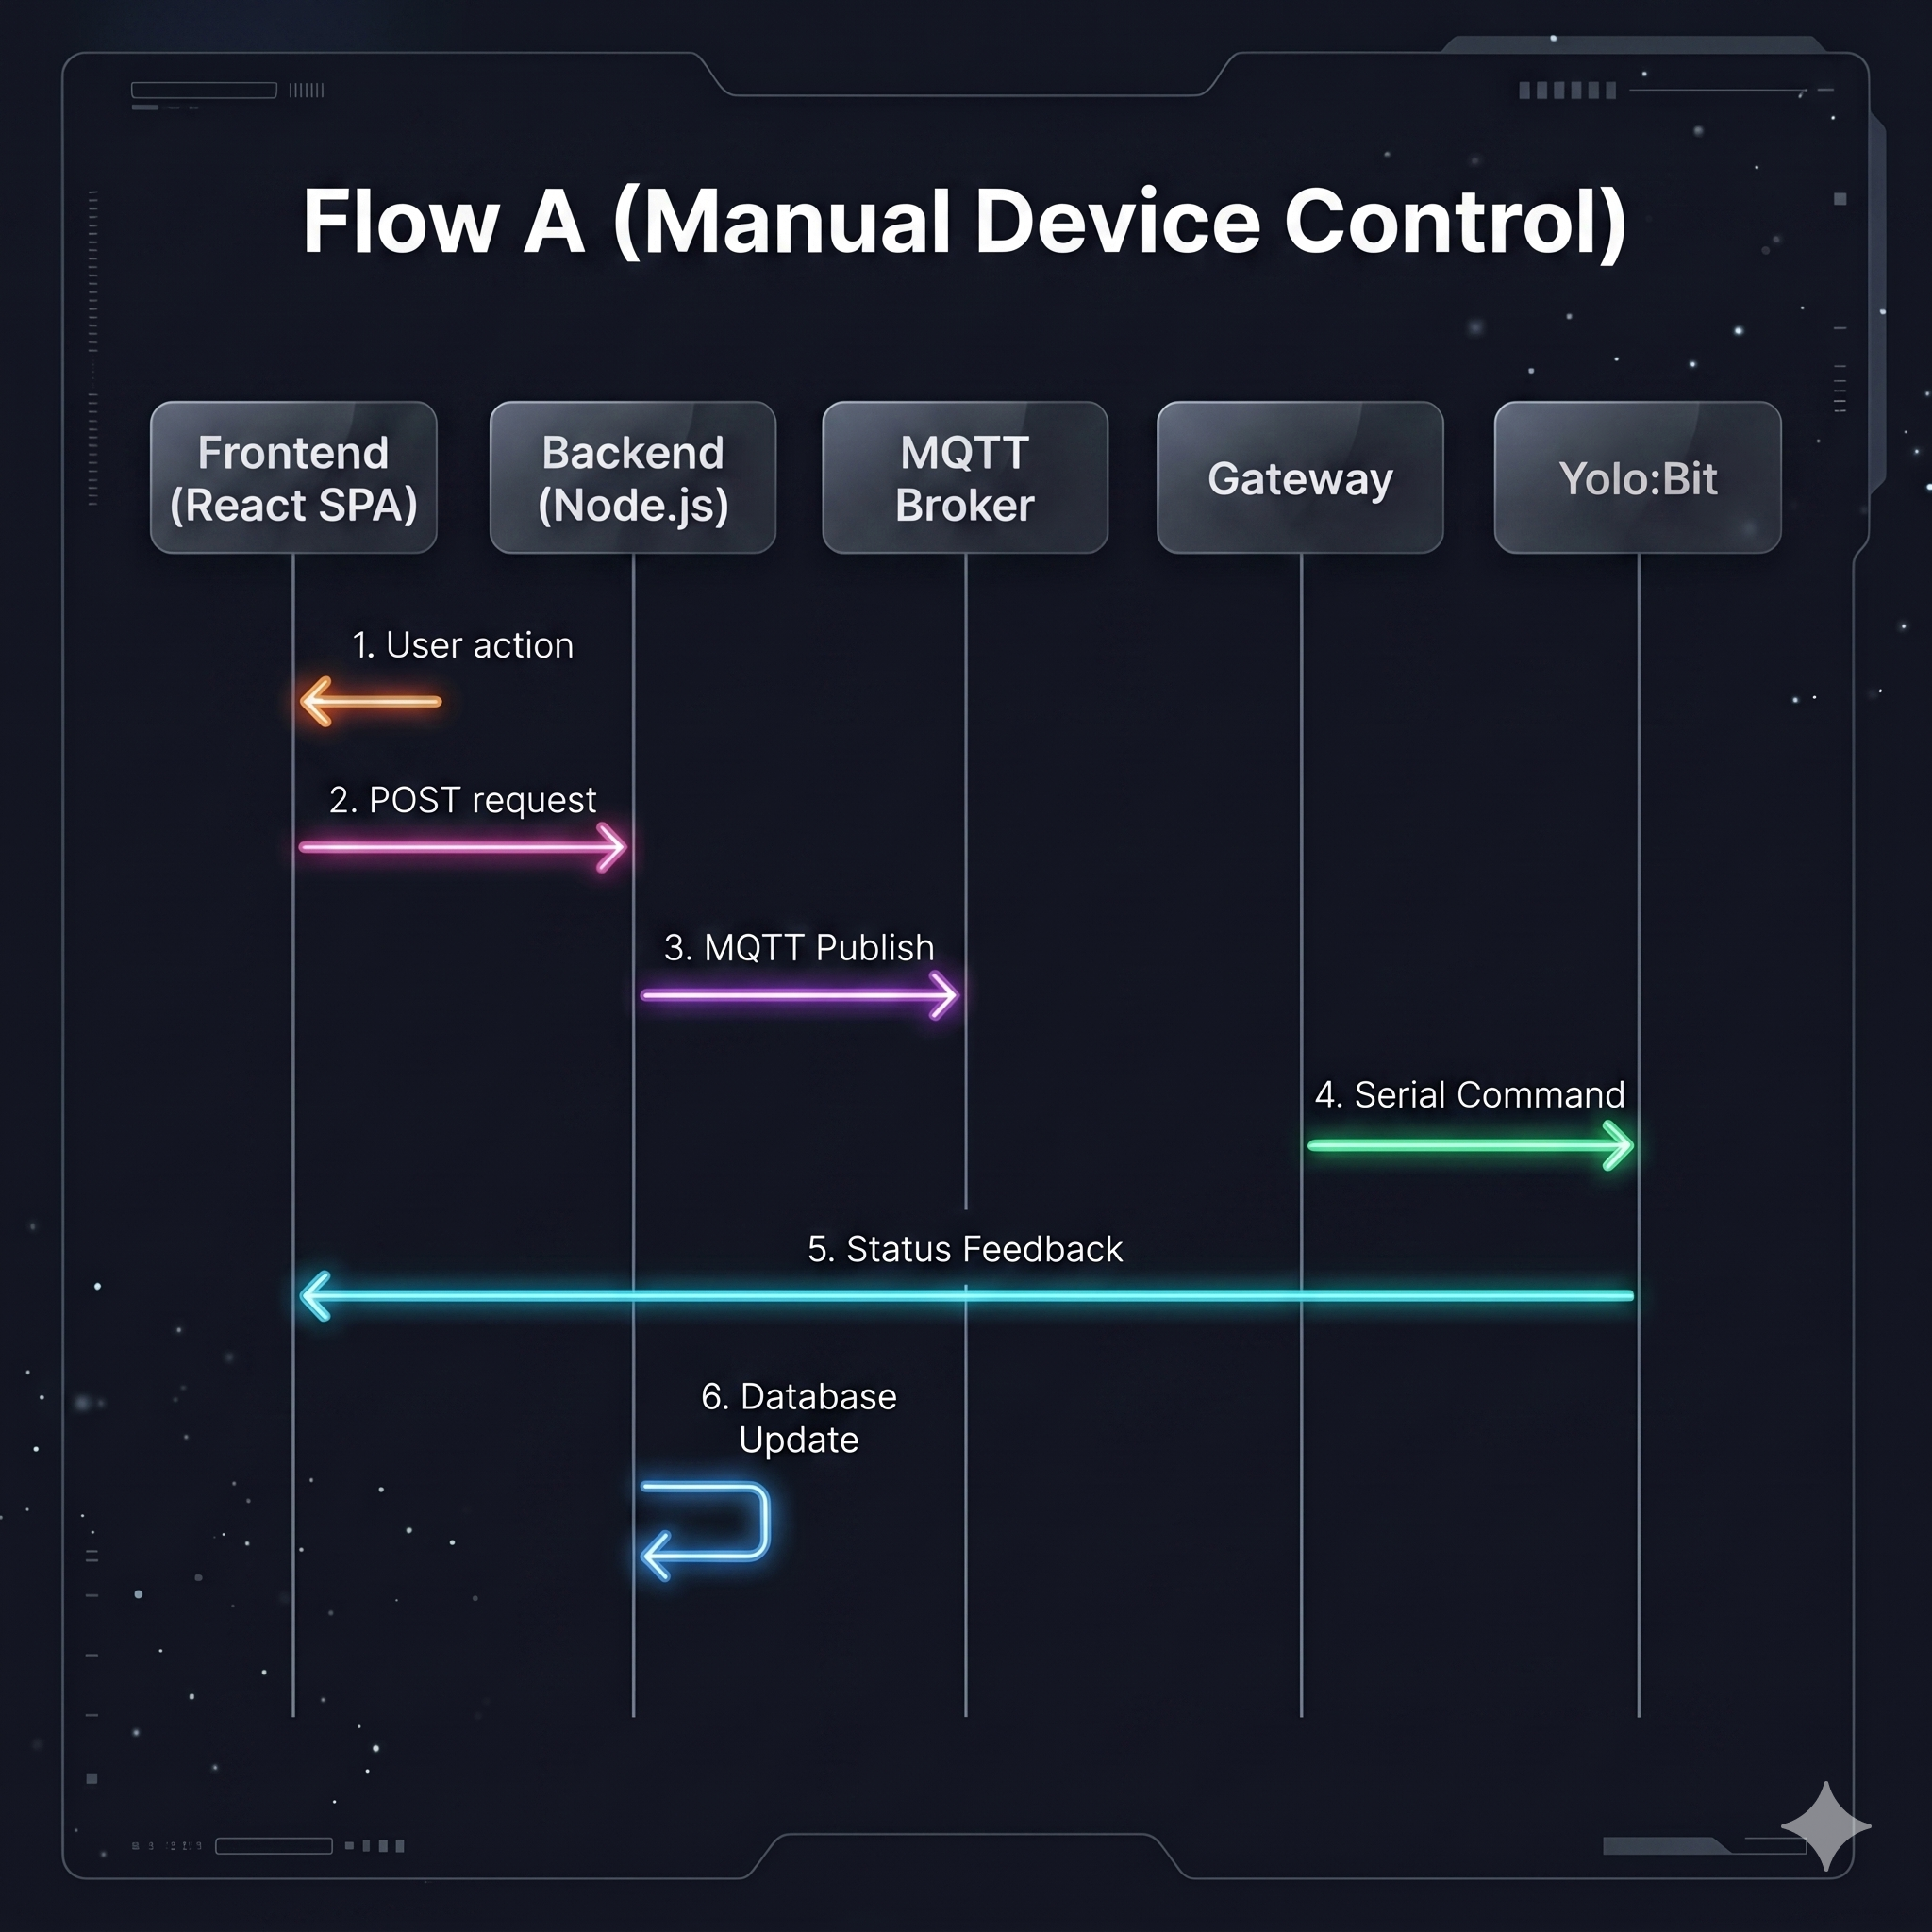
\includegraphics[width=0.95\textwidth]{figures/flow-a-dieu-khien.png}
    \caption{Lược đồ tuần tự luồng điều khiển thiết bị thủ công (Flow A)}
    \label{fig:flow-a-dieu-khien}
\end{figure}

\paragraph{Luồng hoạt động B: Thu thập cảm biến và Cảnh báo ngưỡng}
Kit Yolo:Bit đo đạc liên tục các thông số vật lý của môi trường thông qua các cảm biến nhiệt độ, độ ẩm và ánh sáng. Định kỳ, các thông số này được đóng gói và truyền lên Gateway Python dưới dạng các khung Serial nhỏ. Gateway bóc tách, biên dịch và đăng tải (publish) các thông số lên các topic MQTT tương ứng. Backend Express lắng nghe, tích lũy các chỉ số vào bộ đệm snapshot. Khi nhận đủ 3 chỉ số, Backend tiến hành ghi snapshot cảm biến vào MongoDB và kiểm tra tính an toàn dựa trên tập cấu hình ngưỡng để chủ động sinh cảnh báo và tự động kích hoạt thiết bị phần cứng để khắc phục sự cố.

% Mermaid Source Code cho Flow B:
% sequenceDiagram
%   autonumber
%   participant KIT as Yolo:Bit kit
%   participant GW as Gateway
%   participant MQTT as Mosquitto
%   participant BE as Backend
%   participant DB as MongoDB
%   participant UI as Frontend Dashboard
% 
%   KIT->>GW: Serial "!T:31#" "!H:55#" "!Lu:200#"
%   GW->>MQTT: publish home/livingroom/sensor/{temperature,humidity,light} {"value":"31"} ...
%   MQTT->>BE: deliver (one per sensor)
%   BE->>BE: handleSensorTelemetry → buffer
%   Note over BE: When all 3 sensors present →
%   BE->>DB: SensorService.saveSensorSnapshot()
%   BE->>BE: alertService.checkAndAlert("temperature",31)
%   BE->>BE: rule temp.above=30 violated · no active dup
%   BE->>DB: Alert.create({type:"temperature", severity:"WARNING", value:31, threshold:30, condition:">"})
%   BE->>DB: ThresholdTrace.create(...) (fire-and-forget)
%   UI->>BE: GET /api/alerts/active (poll every 5s)
%   BE-->>UI: {data:[Alert]}
%   UI->>UI: render alert card, translate to VN
%   UI->>BE: PATCH /api/alerts/:id/resolve
%   BE->>DB: isResolved=true, resolvedAt=now
%   BE-->>UI: {success:true, data:Alert}
%   UI->>UI: remove alert from list
\begin{figure}[H]
    \centering
    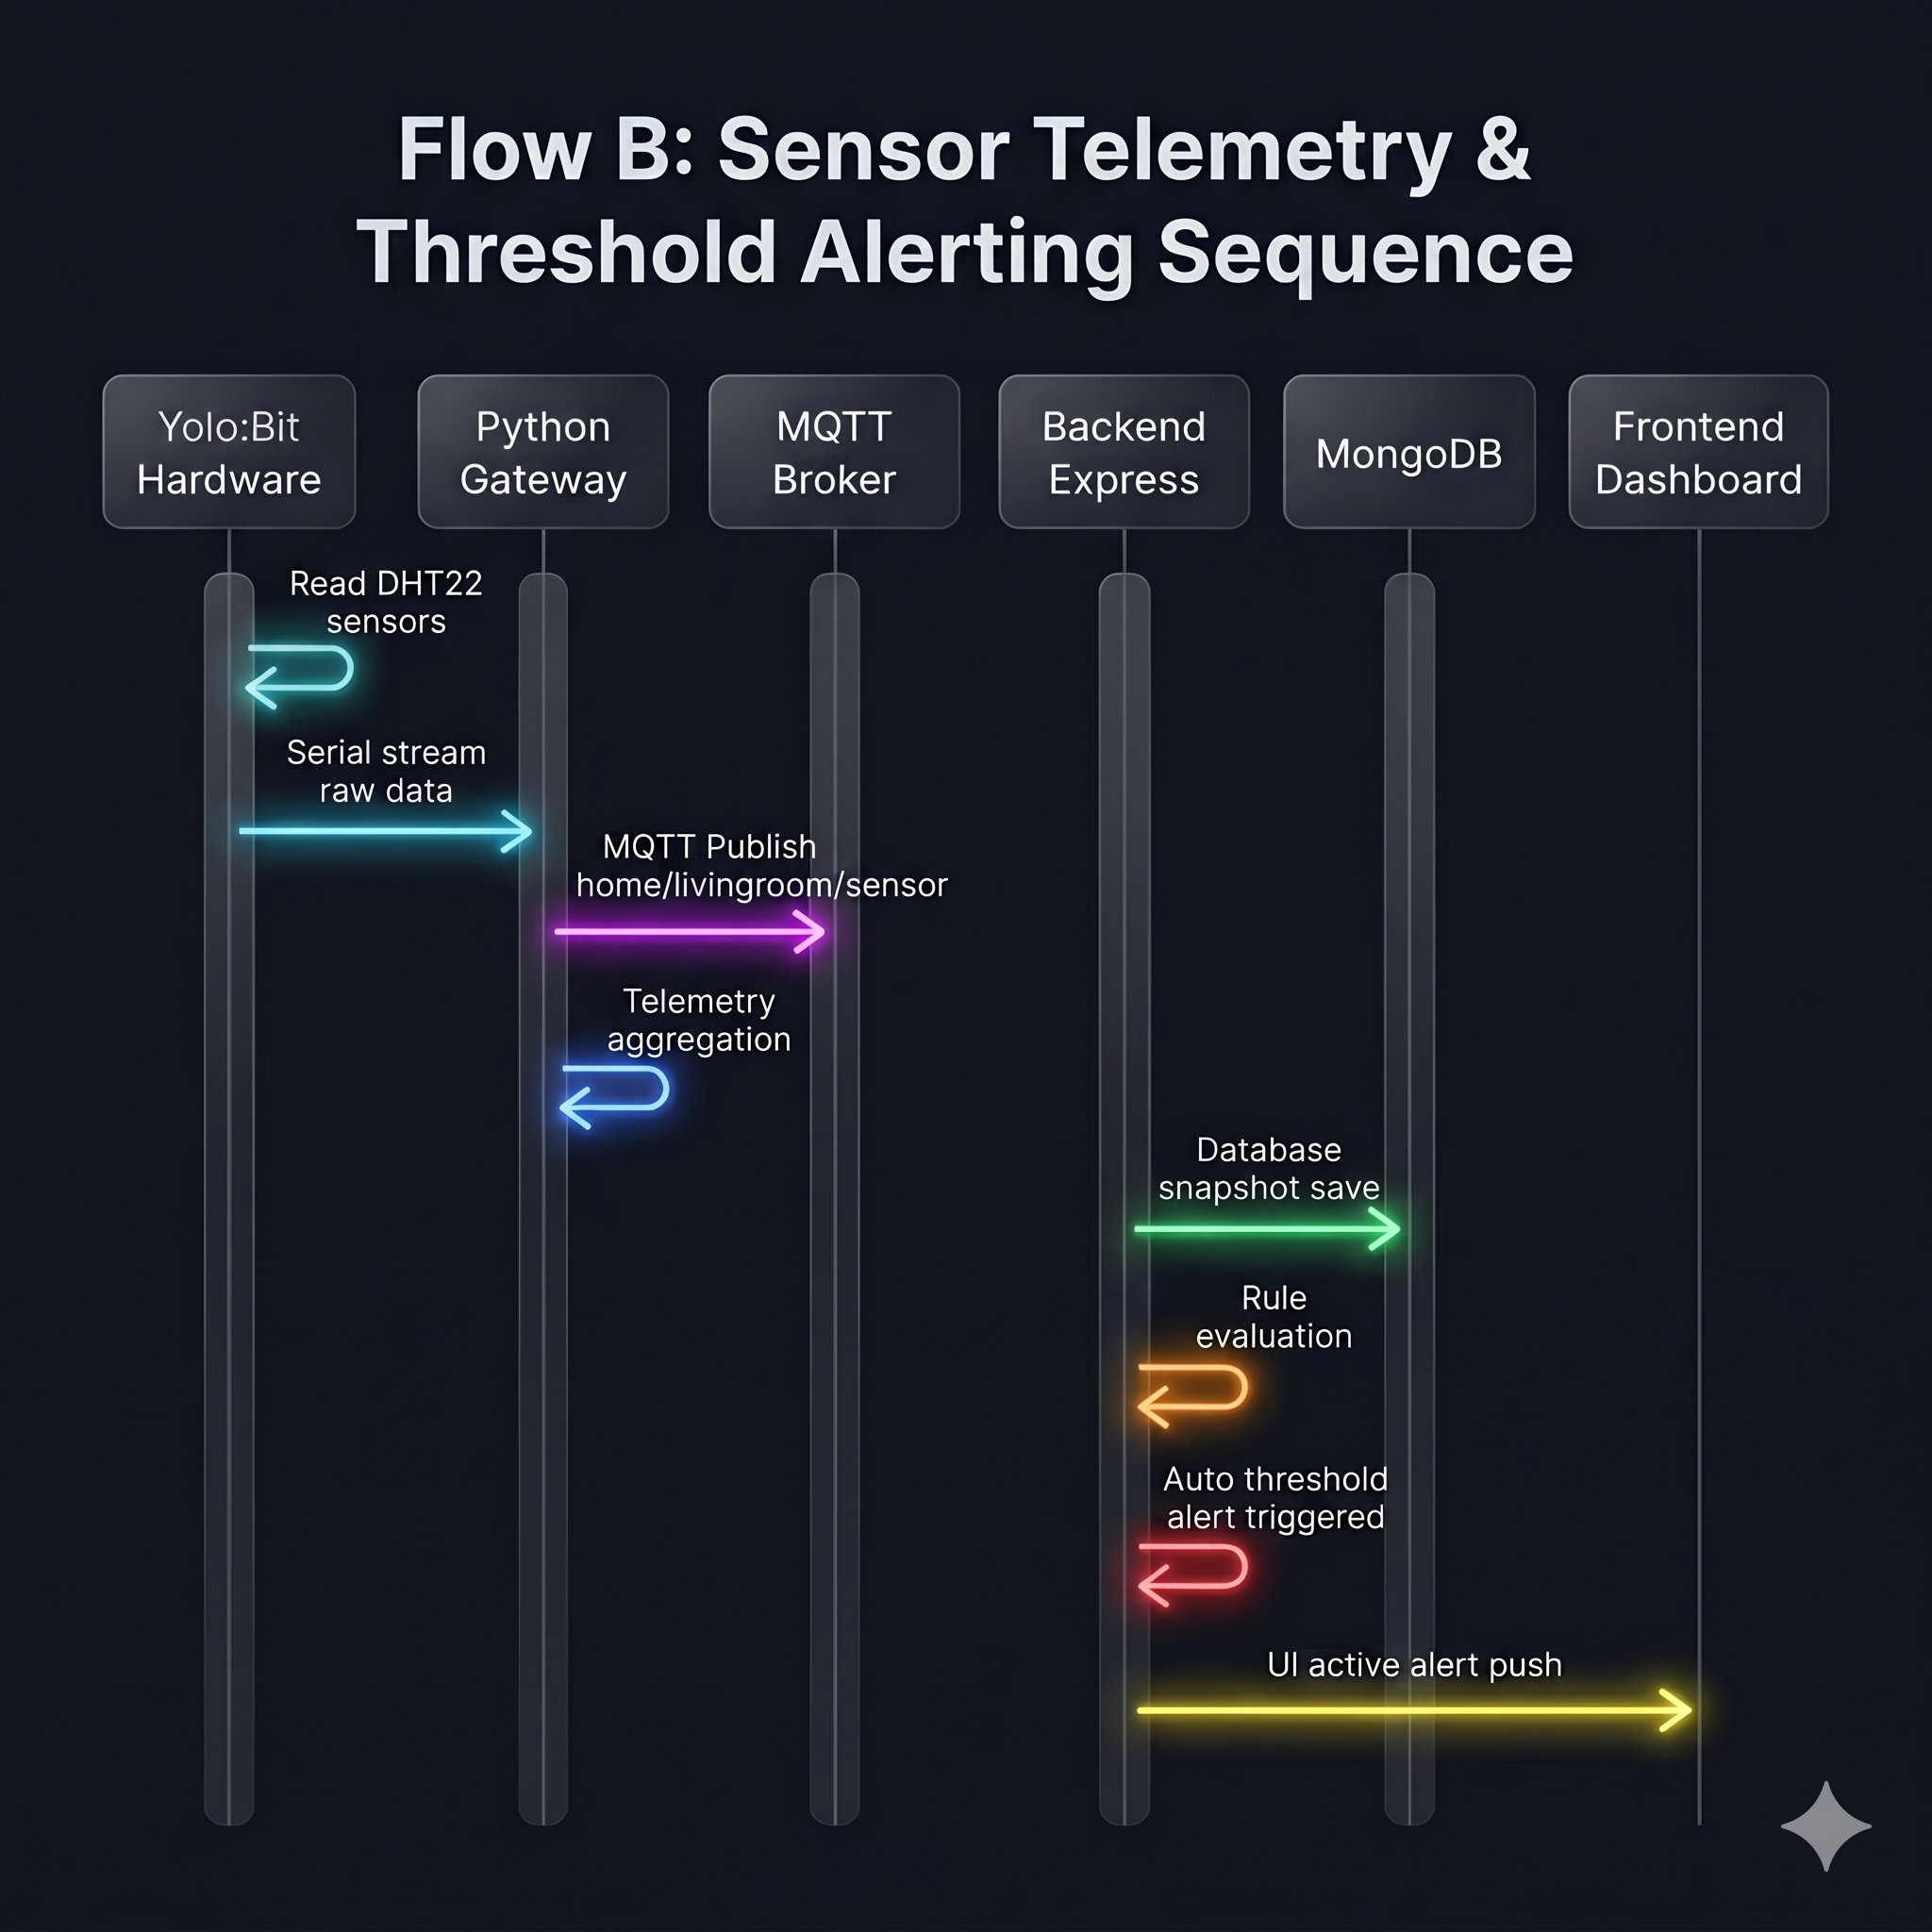
\includegraphics[width=0.95\textwidth]{figures/flow-b-canh-bao.png}
    \caption{Lược đồ tuần tự luồng thu thập cảm biến và xử lý cảnh báo ngưỡng (Flow B)}
    \label{fig:flow-b-canh-bao}
\end{figure}

\paragraph{Luồng hoạt động C: Điều khiển bằng giọng nói}
Khi người dùng tương tác bằng giọng nói trên giao diện Web (Push-to-Talk), trình duyệt sử dụng thư viện RecordRTC ghi âm luồng tiếng nói định dạng mono WAV tần số 16kHz gửi POST lên Backend. Backend Express tiếp nhận file âm thanh, chuyển tiếp qua luồng nhị phân tới dịch vụ Vosk STT (cổng 8500) để nhận dạng văn bản tiếng Việt. Chuỗi văn bản sau đó được gửi tiếp tới dịch vụ ML (cổng 8000) để phân loại ý định thành định dạng lệnh chuẩn. Backend nhận kết quả phân tích, tiến hành chuẩn hóa lệnh rồi xuất bản bản tin MQTT xuống Gateway để điều khiển thiết bị vật lý, đồng thời phản hồi kết quả trực quan dạng Toast trên màn hình Web.

% Mermaid Source Code cho Flow C:
% sequenceDiagram
%   autonumber
%   participant USER as User
%   participant VC as VoiceControl (browser)
%   participant BE as Backend (/api/voice/command)
%   participant VOSK as Vosk :8500
%   participant ML as ML :8000
%   participant MQTT as Mosquitto
%   participant GW as Gateway
%   participant KIT as Yolo:Bit kit
% 
%   USER->>VC: press-and-hold mic button
%   VC->>VC: RecordRTC start (mono 16kHz WAV)
%   USER->>VC: release
%   VC->>BE: POST /api/voice/command (multipart "audio")
%   BE->>VOSK: POST /transcribe (field "file")
%   VOSK-->>BE: {transcript:"bật đèn"}
%   BE->>ML: POST /predict {text:"bật đèn"}
%   ML-->>BE: {intent:"led:on"}
%   BE->>BE: normalizeIntent → {device:"led",action:"on"}
%   BE->>MQTT: publish home/default/device/led/set {"action":"on"}
%   Note over BE,MQTT: location defaults to "default" — diverges from gateway's livingroom subscriptions; see §6.5
%   BE-->>VC: {status:"success", data:{transcript, intent}}
%   VC->>VC: show toast 5 s
%   MQTT->>GW: (if topic matches subscription)
%   GW->>KIT: Serial "!L:1#"
\begin{figure}[H]
    \centering
    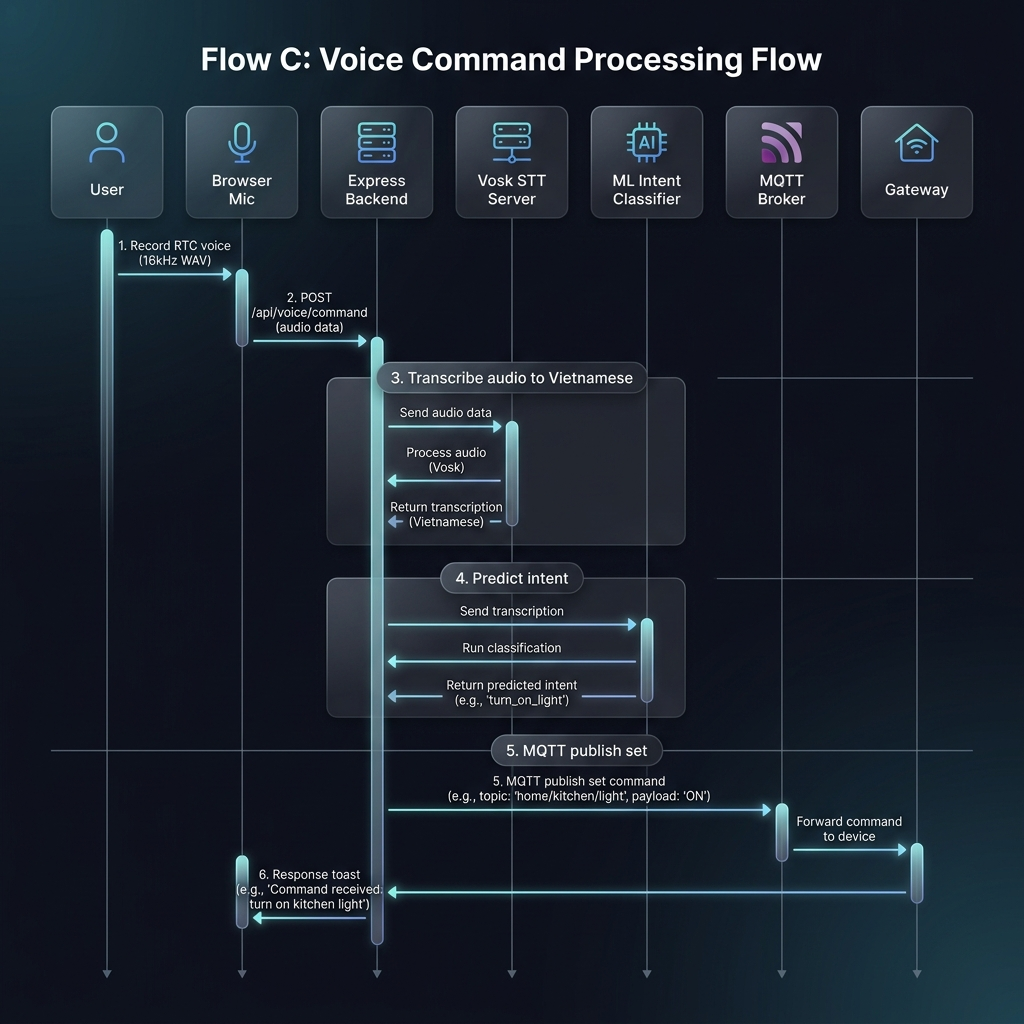
\includegraphics[width=0.95\textwidth]{figures/flow-c-giong-noi.png}
    \caption{Lược đồ tuần tự luồng điều khiển bằng giọng nói tiếng Việt (Flow C)}
    \label{fig:flow-c-giong-noi}
\end{figure}

\subsection{Module 1 --- Đo đạc và hiển thị môi trường}

\subsubsection{Mục tiêu}
Đo lường các chỉ số môi trường sống thực tế bao gồm nhiệt độ, độ ẩm và cường độ ánh sáng trong nhà, sau đó gửi dữ liệu thu thập lên hệ thống và hiển thị trực quan các giá trị này lên giao diện Web Dashboard của người dùng theo thời gian thực để hỗ trợ giám sát an toàn.

\subsubsection{Thành phần liên quan}
Các thành phần và tệp tin mã nguồn tham gia trực tiếp vào module bao gồm:
\begin{itemize}
    \item \textbf{Giao diện Frontend}: \texttt{Dashboard.js} (dòng 6--10, 37--59, 75, 128--149) chịu trách nhiệm tạo trạng thái lưu dữ liệu cảm biến, xây dựng hàm gọi API và thiết lập chu kỳ polling tự động.
    \item \textbf{Dịch vụ Backend Node.js}: \texttt{sensor.js} (router GET \texttt{/api/sensors/latest}), \texttt{sensorController.js} (dòng 5--15), \texttt{sensorService.js} (dòng 5--8) và \texttt{mqttService.js} (dòng 152--199) để xử lý định tuyến, truy vấn cơ sở dữ liệu MongoDB và gom dữ liệu cảm biến MQTT.
    \item \textbf{Dịch vụ Python Gateway}: \texttt{run.py} (dòng 244--246) để chạy luồng đọc Serial nền, \texttt{controller.py} (dòng 291--333) để phân tích khung truyền Serial và \texttt{default\_adapter.py} (dòng 53--73) để biên dịch ánh xạ cổng cảm biến.
    \item \textbf{Cấu hình tệp tin}: \texttt{config.yml} (dòng 75--78) cấu hình các ký tự viết tắt tương ứng với tên cổng cảm biến.
\end{itemize}

\subsubsection{Luồng xử lý}
Luồng thu thập và hiển thị cảm biến môi trường được xử lý qua 8 bước cụ thể như mô tả trong lược đồ tuần tự của \autoref{fig:flow-b-canh-bao}:
\begin{itemize}
    \item Hệ thống phần cứng Kit Yolo:Bit đo đạc các giá trị vật lý và định kỳ truyền lên Gateway Python qua kết nối cáp USB Serial dạng chuỗi ký tự viết tắt liên tục, ví dụ: \texttt{!T:27.5\#!H:60\#!Lu:350\#}.
    \item Luồng đọc nền Serial của Gateway Python (\texttt{run.py}) lắng nghe cổng COM vật lý và chuyển chuỗi nhận được cho hàm \texttt{MainController.\_on\_serial}.
    \item Bộ phân tích cú pháp của Gateway sử dụng biểu thức chính quy tách chuỗi thành các khung truyền con có dạng cấu trúc \texttt{!<ABBR>:<VALUE>\#}.
    \item Hàm chuyển đổi \texttt{DefaultDataAdapter.from\_serial} biên dịch các mã viết tắt cổng (\texttt{T}, \texttt{H}, \texttt{Lu}) thành tên cảm biến tiếng Anh tương thích (\texttt{temperature}, \texttt{humidity}, \texttt{light}) dựa trên cấu hình trong \texttt{config.yml}.
    \item Gateway thực hiện xuất bản (publish) dữ liệu JSON thô lên Broker MQTT Mosquitto với cấu trúc topic chuẩn, ví dụ: \texttt{home/livingroom/sensor/temperature} chứa payload \texttt{\{"value": "27.5"\}}.
    \item Backend Node.js nhận được tin nhắn qua dịch vụ \texttt{mqttService.js}, trích xuất giá trị số và đưa vào bộ đệm gom snapshot tạm thời có tên \texttt{sensorSnapshotBuffer}.
    \item Khi bộ đệm gom đầy đủ cả 3 thông số nhiệt độ, độ ẩm và cường độ ánh sáng, Backend gọi \texttt{SensorService.saveSensorSnapshot} ghi dữ liệu snapshot môi trường hoàn chỉnh vào MongoDB và xóa sạch bộ đệm để bắt đầu chu kỳ tiếp theo.
    \item Trình duyệt của người dùng tại giao diện Dashboard liên tục gọi HTTP GET đồng bộ tới endpoint \texttt{/api/sensors/latest} mỗi 5 giây thông qua hàm \texttt{setInterval}. Dữ liệu snapshot mới nhất nhận về được cập nhật lên state và tự động vẽ lại các thẻ hiển thị trên giao diện.
\end{itemize}

\subsubsection{Giao diện người dùng}
Trạng thái hiển thị dữ liệu cảm biến được tích hợp trực quan trên trang Dashboard chính (\texttt{/dashboard}). Giao diện hiển thị bao gồm lưới 3 thẻ (cards) riêng biệt: thẻ Nhiệt độ (hiển thị đơn vị $^\circ$C), thẻ Độ ẩm (hiển thị đơn vị \%) và thẻ Cường độ ánh sáng (hiển thị đơn vị lx) như mô tả tại nhãn hình ảnh \autoref{fig:ui-dashboard}.

\subsubsection{Hạn chế và hướng phát triển}
Hạn chế thiết kế cốt lõi trong Module 1 nằm ở \textbf{cơ chế gom snapshot cảm biến cứng nhắc}. Vì Backend Node.js chỉ thực hiện ghi nhận dữ liệu vào MongoDB và kiểm tra tự động hóa khi bộ đệm \texttt{sensorSnapshotBuffer} có đầy đủ cả 3 thông số cảm biến môi trường gửi lên, hệ thống sẽ gặp lỗi treo cứng (deadlock) nếu một trong các cảm biến vật lý trên phần cứng bị hỏng hoặc ngừng gửi tin nhắn. Trong trường hợp đó, toàn bộ dữ liệu môi trường sẽ không bao giờ được cập nhật tiếp vào cơ sở dữ liệu và các logic tự động hóa cảnh báo phía Backend cũng bị ngưng trệ hoàn toàn. Hướng khắc phục trong tương lai là áp dụng cơ chế timeout cho bộ đệm hoặc lưu trữ các thông số môi trường một cách độc lập kết hợp cơ chế nội suy dữ liệu cũ.

\subsection{Module 2 --- Tự động hóa và cảnh báo ngưỡng}

\subsubsection{Mục tiêu}
Phát hiện các hành vi vi phạm ngưỡng an toàn môi trường dựa trên các tập cấu hình ngưỡng ngày và đêm; Tự động kích hoạt thiết bị tương ứng khi xảy ra vi phạm (như bật quạt khi trời nóng, bật đèn LED khi trời tối); Sinh các thông báo vi phạm hiển thị trên Dashboard và gửi cảnh báo khẩn cấp tới điện thoại của người dùng qua ứng dụng di động.

\subsubsection{Trạng thái cài đặt}
Hoàn thành một phần

\subsubsection{Thành phần liên quan}
Các thành phần mã nguồn tham gia trực tiếp bao gồm:
\begin{itemize}
    \item \textbf{Gateway Python (Tự động hóa vật lý)}: \texttt{controller.py} (dòng 90--113, 327) để phân luồng kiểm tra, \texttt{threshold\_service.py} (dòng 142--192) để so sánh các quy tắc ngưỡng và phát lệnh Serial.
    \item \textbf{Backend Node.js (Cảnh báo an toàn)}: \texttt{mqttService.js} (dòng 185--188) để kích hoạt kiểm tra khi đủ cảm biến, \texttt{alertService.js} (dòng 183--252) để xử lý logic sinh cảnh báo và ngăn cảnh báo trùng lặp.
    \item \textbf{Giao diện Dashboard}: \texttt{Dashboard.js} (dòng 13--18, 151--183) hiển thị khu vực cảnh báo đỏ nổi bật cùng nút bấm giải tỏa thủ công.
    \item \textbf{Tệp cấu hình hệ thống}: \texttt{config.yml} (dòng 49--70) định nghĩa các quy tắc ngưỡng cứng ở Gateway và \texttt{alertService.js} (dòng 33--44) định nghĩa các ngưỡng tĩnh Backend.
\end{itemize}

\subsubsection{Luồng xử lý}
Luồng tự động hóa vật lý và cảnh báo ngưỡng an toàn được thực hiện đồng thời qua hai tuyến xử lý như được biểu diễn trong \autoref{fig:flow-b-canh-bao}:
\begin{itemize}
    \item \textbf{Tuyến tự động hóa cục bộ ở Gateway}:
        \begin{itemize}
            \item Khi nhận được số đo từ cảm biến gửi lên qua Serial (ví dụ: nhiệt độ 32$^\circ$C), \texttt{MainController} của Gateway lập tức chuyển dữ liệu tới \texttt{ThresholdService}.
            \item \texttt{ThresholdService} duyệt qua tập cấu hình rules trong \texttt{config.yml}. Đối chiếu nhiệt độ $32 > 30$ (ngưỡng trên của quạt Fan), hệ thống xác định quy tắc bị vi phạm.
            \item Để tránh gửi lệnh vật lý dồn dập, Gateway so sánh trạng thái trước đó. Nếu quạt đang tắt, Gateway sinh khung lệnh \texttt{!F:1\#} gửi xuống Yolo:Bit để bật quạt vật lý và lưu vết vào Database.
        \end{itemize}
    \item \textbf{Tuyến sinh cảnh báo an toàn trên Backend Express}:
        \begin{itemize}
            \item Sau khi gom đủ snapshot cảm biến thành công, Backend gọi hàm kiểm tra \texttt{alertService.checkAndAlert}.
            \item Hàm này so sánh giá trị cảm biến thực tế với cấu hình ngưỡng trong tệp tin. Nếu phát hiện vi phạm, hệ thống kiểm tra trong bộ sưu tập \texttt{Alert} xem có cảnh báo cùng loại nào đang mở (\texttt{isResolved: false}) hay không.
            \item Nếu chưa tồn tại cảnh báo chủ động, Backend Express chèn bản ghi cảnh báo mới vào MongoDB, đồng thời lưu nhật ký dấu vết tự động \texttt{ThresholdTrace}.
            \item Trình duyệt của người dùng thực hiện polling API \texttt{GET /api/alerts/active} mỗi 5 giây và hiển thị hộp thông tin màu đỏ cảnh báo trên màn hình.
            \item Người dùng nhấn nút "Xác nhận" để gửi lệnh \texttt{PATCH /api/alerts/:id/resolve} lên Backend, cập nhật trạng thái \texttt{isResolved = true} trên MongoDB, làm biến mất hộp cảnh báo trên Dashboard.
        \end{itemize}
\end{itemize}

\subsubsection{Giao diện người dùng}
Trình duyệt người dùng kết xuất thành phần "Cảnh báo ngưỡng" nổi bật có màu đỏ ở phía dưới khu vực hiển thị các thẻ cảm biến môi trường trên Dashboard. Mỗi thông báo vi phạm chứa tên cảm biến được dịch hóa hoàn toàn sang tiếng Việt (ví dụ: "Nhiệt độ", "Độ ẩm", "Ánh sáng") cùng mô tả chi tiết giá trị thực đo so với ngưỡng an toàn quy định và có một nút bấm màu đỏ nhãn "Xác nhận" để giải tỏa cảnh báo (Tham chiếu: \autoref{fig:ui-alert}).

\subsubsection{Hạn chế và hướng phát triển}
Module 2 hiện tại tồn tại hai khoảng trống thiết kế vô cùng nghiêm trọng cần ghi nhận một cách thực chứng:
\begin{itemize}
    \item \textbf{Hoàn toàn thiếu tự động điều chỉnh ngưỡng theo ngày/đêm}: Hệ thống chỉ sử dụng một tập cấu hình ngưỡng tĩnh hoạt động cố định từ tệp tin cấu hình. Mã nguồn hoàn toàn không chứa bất kỳ logic kiểm tra múi giờ, lấy thời gian thực từ hệ thống hay lập lịch (cron job) để chuyển đổi qua lại giữa hai chế độ cấu hình ngày/đêm.
    \item \textbf{Hoàn toàn thiếu cảnh báo qua ứng dụng di động}: Không có bất kỳ dòng mã nào liên quan đến các nhà cung cấp dịch vụ gửi thông báo đẩy di động như Firebase Cloud Messaging (FCM), OneSignal hay tin nhắn SMS Twilio. Hệ thống hoàn toàn phụ thuộc vào việc polling giao diện web, điều này làm mất đi khả năng thông báo tức thời của một hệ thống an toàn chuyên nghiệp.
\end{itemize}
Hướng phát triển tiếp theo là xây dựng luồng thời gian thực cho phép Gateway tải lại cấu hình ngưỡng dựa trên bộ lập lịch giờ tự động và tích hợp gói SDK FCM của Firebase vào Backend Node.js để gửi thông báo khẩn tới điện thoại người dùng.

\subsection{Module 3 --- Giao diện điều khiển thiết bị}

\subsubsection{Mục tiêu}
Thiết kế giao diện người dùng trên ứng dụng Web cho phép người dùng giám sát trạng thái và chủ động bật/tắt thủ công từ xa các thiết bị điện trong gia đình bao gồm đèn chiếu sáng (LED), quạt thông gió (Fan) và động cơ rèm cửa (Servo).

\subsubsection{Trạng thái cài đặt}
Đã hoàn thành

\subsubsection{Thành phần liên quan}
Các thành phần mã nguồn tham gia điều phối trực tiếp luồng bật/tắt thiết bị bao gồm:
\begin{itemize}
    \item \textbf{Trình duyệt Frontend}: \texttt{DeviceManagement.js} (dòng 46--77, 143--170) và \texttt{api.js} (dòng 25--39) chịu trách nhiệm kết xuất giao diện thẻ bật/tắt và gửi yêu cầu REST.
    \item \textbf{Backend Express}: \texttt{device.js} (router POST \texttt{/api/devices/control}), \texttt{deviceController.js} (dòng 24--118) và \texttt{mqttService.js} (dòng 309--339) tiếp nhận yêu cầu, cập nhật MongoDB, lưu vết lịch sử điều khiển và đẩy lệnh lên MQTT.
    \item \textbf{Gateway Python}: \texttt{controller.py} (dòng 215--290) tiếp nhận thông tin điều khiển từ MQTT, giải mã và viết trực tiếp xuống cổng truyền Serial vật lý.
\end{itemize}

\subsubsection{Luồng xử lý}
Luồng điều khiển thiết bị thủ công được thực thi theo 7 bước tuần tự tương thích với lược đồ tuần tự của \autoref{fig:flow-a-dieu-khien}:
\begin{itemize}
    \item Người dùng nhấp chuột vào công tắc gạt trạng thái trên thẻ thiết bị (ví dụ: LED) trên trang Quản lý thiết bị của trình duyệt.
    \item Trình duyệt lập tức gửi yêu cầu HTTP POST đồng bộ tới Backend thông qua endpoint \texttt{/api/devices/control} chứa payload \texttt{\{deviceName: "led", action: "on", deviceType: "led"\}}.
    \item Backend Express nhận yêu cầu, tiến hành kiểm tra nghiệp vụ và ghi nhận bản ghi nhật ký điều khiển thủ công vào cơ sở dữ liệu MongoDB dưới dạng một tài liệu \texttt{ControlTrace}.
    \item Backend gọi hàm \texttt{mqttService.sendDeviceCommand} để xuất bản bản tin lệnh JSON \texttt{\{"action": "on"\}} tới topic MQTT \texttt{home/livingroom/device/led/set}. Đồng thời, Backend cập nhật tạm thời trạng thái thiết bị LED thành \texttt{"on"} trong snapshot gần nhất để giao diện đồng bộ tức thời.
    \item Gateway Python lắng nghe topic lệnh qua cầu nối \texttt{mqtt\_client.py}, gọi hàm \texttt{\_on\_mqtt} trong \texttt{MainController} để dịch chuyển trạng thái điều khiển thành giá trị nhị phân kỹ thuật (\texttt{on} $\rightarrow$ \texttt{1}).
    \item Gateway truyền khung ký tự Serial \texttt{!L:1\#} xuống Kit Yolo:Bit thông qua cổng UART. Kit Yolo:Bit nhận lệnh, tác động Relay cấp nguồn cho đèn sáng vật lý và phản hồi ngược lại chuỗi \texttt{!L:1\#} qua UART để xác nhận.
    \item Gateway Python tiếp nhận phản hồi, đẩy trạng thái chính thức lên topic MQTT \texttt{home/livingroom/device/led/state} để Backend Express thu thập và đồng bộ snapshot thiết bị lâu dài vào cơ sở dữ liệu MongoDB.
\end{itemize}

\subsubsection{Giao diện người dùng}
Trang Quản lý thiết bị (\texttt{/devices}) hiển thị nhãn tiêu đề "Các thiết bị được kết nối" và kết xuất lưới các thẻ điều khiển thiết bị bao gồm Đèn LED, Quạt và Rèm cửa động cơ Servo. Mỗi thẻ thiết bị hiển thị biểu tượng trạng thái cùng một công tắc gạt ngang để người dùng thao tác. Khi thiết bị được bật thành công, thẻ chuyển màu nền sáng nổi bật kèm nhãn hiển thị trạng thái "Active" (Tham chiếu: \autoref{fig:ui-devices}).

\subsubsection{Hạn chế và hướng phát triển}
Module 3 hoạt động ổn định và có độ trễ phản hồi phần cứng cực thấp nhờ sự kết hợp giữa MQTT và truyền tải Serial UART. Không phát hiện khoảng trống thiết kế nghiêm trọng nào ảnh hưởng đến trải nghiệm điều khiển thủ công cơ bản. Hướng phát triển tiếp theo là bổ sung cơ chế xác thực mã hóa hai đầu cho khung truyền Serial để ngăn chặn các cuộc tấn công tiêm lệnh trái phép từ các thiết bị Serial giả mạo.

\subsection{Module 4 --- Lưu trữ lịch sử và ghi sự kiện}

\subsubsection{Mục tiêu}
Lưu trữ bền vững lịch sử hoạt động đo đạc của cảm biến môi trường và trạng thái thiết bị theo thời gian; Ghi nhật ký chi tiết các sự kiện vận hành hệ thống bao gồm: tương tác thủ công của người dùng trên Web, quá trình xử lý giọng nói và các tác động tự động hóa do vi phạm ngưỡng kích hoạt.

\subsubsection{Trạng thái cài đặt}
Hoàn thành một phần

\subsubsection{Thành phần liên quan}
Các cấu trúc lưu trữ và mã nguồn ghi sự kiện bao gồm:
\begin{itemize}
    \item \textbf{Cơ sở dữ liệu lưu trữ snapshot}: \texttt{mqttService.js} (dòng 138, 178) thực hiện gọi dịch vụ lưu trữ dữ liệu môi trường và thiết bị định kỳ vào MongoDB.
    \item \textbf{Nhật ký tương tác người dùng (Manual \& Voice)}: \texttt{deviceController.js} (dòng 93--100) và \texttt{voiceService.js} (dòng 210, 217) gọi cơ chế chèn vết \texttt{ControlTrace}.
    \item \textbf{Nhật ký tự động hóa (Threshold logic)}: \texttt{alertService.js} (dòng 239--250) thực hiện gọi chèn vết tự động \texttt{ThresholdTrace}.
    \item \textbf{Cấu trúc Schema MongoDB}: \texttt{Sensor.js}, \texttt{Device.js}, \texttt{ControlTrace.js} và \texttt{ThresholdTrace.js} định nghĩa cấu trúc bảng dữ liệu.
\end{itemize}

\subsubsection{Luồng xử lý}
Hệ thống lưu giữ lịch sử hoạt động bền vững thông qua 4 quy trình chạy nền liên tục:
\begin{itemize}
    \item \textbf{Ghi lịch sử cảm biến định kỳ}: Khi Gateway Python đăng tải các số đo thô lên MQTT và Backend Express gom đủ snapshot môi trường thành công, hệ thống tự động ghi bản ghi mới vào bộ sưu tập \texttt{sensors} kèm nhãn thời gian thực tế.
    \item \textbf{Lưu vết tương tác thủ công}: Mọi yêu cầu HTTP POST gửi tới \texttt{deviceController} đều được xử lý và chèn một tài liệu mới vào bộ sưu tập \texttt{control\_traces} chứa các trường thông tin: \texttt{source: "frontend"}, tên \texttt{action} lệnh, \texttt{payload} truyền lên, và cờ \texttt{status} báo cáo thành công hay thất bại.
    \item \textbf{Lưu vết điều khiển giọng nói}: Khi người dùng ra lệnh bằng tiếng nói, dịch vụ \texttt{voiceService.js} ghi nhận chuỗi văn bản dịch nghĩa và intent ML tương ứng chèn vào bộ sưu tập \texttt{control\_traces} với \texttt{source: "api-client"}.
    \item \textbf{Ghi vết tự động hóa do vượt ngưỡng}: Khi Gateway hoặc Backend thực thi lệnh khẩn cấp kích hoạt thiết bị để bảo vệ hệ thống do vi phạm ngưỡng an toàn (ví dụ: bật quạt khi nóng quá mức), \texttt{alertService.js} chèn nhật ký vào bộ sưu tập \texttt{threshold\_traces} lưu thông tin về loại cảm biến vi phạm, giá trị đo đạc, ngưỡng an toàn và trạng thái thiết bị bị thay đổi.
\end{itemize}

\subsubsection{Giao diện người dùng}
\textbf{Hệ thống hoàn toàn không có giao diện người dùng phục vụ chức năng xem lịch sử hay sự kiện}. Ứng dụng Web chỉ cung cấp trang Dashboard hiện hành và trang Thiết bị, thanh điều hướng Sidebar hoàn toàn thiếu các thẻ liên kết để mở trang Xem đồ thị lịch sử cảm biến, Lịch sử cảnh báo hay Nhật ký hệ thống (log viewer). Người dùng không thể xem lại các dấu vết lịch sử nếu không truy cập trực tiếp vào MongoDB thông qua các công cụ kỹ thuật như MongoDB Compass.

\subsubsection{Hạn chế và hướng phát triển}
Hạn chế thiết kế vô cùng lớn của Module 4 là \textbf{sự thiếu vắng hoàn toàn của giao diện tương tác lịch sử và API truy vấn lịch sử}. Mặc dù mã nguồn Backend chèn các dấu vết \texttt{ControlTrace} và \texttt{ThresholdTrace} cực kỳ đầy đủ vào cơ sở dữ liệu MongoDB, hệ thống lại hoàn toàn thiếu các API phục vụ tìm kiếm phân trang dữ liệu lịch sử và thiếu giao diện hiển thị (như trang báo cáo, biểu đồ đường lịch sử biến thiên nhiệt độ/độ ẩm Recharts trên Web). Người dùng thông thường không có cách nào tiếp cận các thông tin lịch sử hoạt động hữu ích này. Hướng phát triển là bổ sung các API phân trang tại Backend Express và thiết kế thêm màn hình Lịch sử tích hợp biểu đồ trực quan giúp người dùng theo dõi và xuất báo cáo.

\subsection{Module 5 --- Điều khiển bằng giọng nói và gợi ý thông minh}

\subsubsection{Mục tiêu}
Tích hợp khả năng ghi âm giọng nói tiếng Việt từ giao diện người dùng, sử dụng các dịch vụ trí tuệ nhân tạo để dịch âm thanh thành văn bản và phân loại ý định để điều khiển thiết bị; Đồng thời, tự động phân tích dữ liệu môi trường để đưa ra các gợi ý đề xuất đóng/mở rèm cửa và cửa sổ thông qua mô hình cây quyết định Decision Tree.

\subsubsection{Thành phần liên quan}
Các thành phần và mã nguồn xử lý luồng AI bao gồm:
\begin{itemize}
    \item \textbf{Giao diện Web (PTT)}: \texttt{VoiceControl.js} (dòng 14--25, 72--79, 81--97) xử lý thu âm bằng RecordRTC và hiển thị Toast phản hồi kết quả giọng nói.
    \item \textbf{Backend Express}: \texttt{voiceRoutes.js} (POST \texttt{/api/voice/command}), \texttt{voiceService.js} (dòng 162--220) điều phối luồng gọi AI và xuất bản lệnh MQTT.
    \item \textbf{Dịch vụ phụ trợ AI}: \texttt{vosk\_server.py} (dịch vụ STT cổng 8500) và \texttt{ml\_server.py} (dịch vụ phân loại intent cổng 8000).
    \item \textbf{Mô hình đề xuất tự động (Gateway)}: \texttt{ai\_service.py} (dòng 16--174) xử lý chạy mô hình và \texttt{curtain\_control\_system.py} huấn luyện mô hình cây quyết định Decision Tree (\texttt{curtain\_model.pkl}).
\end{itemize}

\subsubsection{Luồng xử lý}
Luồng xử lý điều khiển bằng giọng nói tiếng Việt được thực hiện theo 7 bước nghiêm ngặt được mô tả tại lược đồ tuần tự của \autoref{fig:flow-c-giong-noi}:
\begin{itemize}
    \item Người dùng nhấn và giữ phím biểu tượng Mic ở chân màn hình Web, nói rõ câu lệnh tiếng Việt (ví dụ: "bật đèn") và nhả chuột.
    \item Trình duyệt sử dụng công cụ RecordRTC lưu luồng ghi âm định dạng mono WAV tần số lấy mẫu chuẩn 16kHz gửi POST lên Backend Express qua API \texttt{/api/voice/command} dưới dạng multipart.
    \item Backend tiếp nhận dữ liệu nhị phân của file âm thanh, chuyển luồng binary này gọi POST tới dịch vụ STT Vosk hoạt động tại cổng \texttt{8500/transcribe} để nhận diện chuỗi văn bản tiếng Việt.
    \item Nhận được chuỗi văn bản tiếng Việt từ Vosk (ví dụ: \texttt{"bật đèn"}), Backend Express tiếp tục gửi yêu cầu POST chứa chuỗi văn bản này tới dịch vụ ML Intent hoạt động tại cổng \texttt{8000/predict}.
    \item Mô hình học máy phân loại văn bản sang định dạng intent kỹ thuật (ví dụ: \texttt{led:on}), Backend chuẩn hóa và ánh xạ thành công lệnh điều khiển tương ứng (\texttt{device: "led", action: "on"}).
    \item Backend thực hiện lưu trữ thông tin sự kiện vào cơ sở dữ liệu MongoDB và xuất bản lệnh điều khiển lên Broker MQTT thông qua chủ đề \texttt{home/default/device/led/set}.
    \item Trình duyệt nhận phản hồi JSON từ Backend và hiển thị một hộp Toast đen mờ trong 5 giây ghi nhận văn bản nhận diện được và ý định hệ thống đang thực thi.
\end{itemize}

\subsubsection{Giao diện người dùng}
Giao diện điều khiển bằng giọng nói được triển khai dưới dạng một nút Microphone trôi nổi (Float component) luôn xuất hiện ở góc dưới bên phải màn hình Web Layout. Khi người dùng nhấp giữ chuột, biểu tượng Micro màu xanh chuyển sang hình ô vuông màu đỏ nhấp nháy phát xung lan tỏa thể hiện trạng thái đang ghi âm. Khi nhả chuột và Backend đang xử lý, nút chuyển sang biểu tượng xoay tải. Sau đó, một hộp Toast kết quả xuất hiện trên góc màn hình ghi nhận chi tiết câu lệnh người dùng nói và ý định hệ thống hiểu được (Tham chiếu: \autoref{fig:ui-voice}).

\subsubsection{Hạn chế và hướng phát triển}
Module 5 hiện tại bộc lộ hai khoảng trống lớn và một lỗi thiết kế nghiêm trọng cản trở quá trình vận hành thực tế:
\begin{itemize}
    \item \textbf{Lỗi không khớp chủ đề điều khiển vị trí (Location Mismatch)}: Đây là một lỗi thiết kế nghiêm trọng trong mã nguồn Backend. Khi dịch nghĩa giọng nói thành công và xuất bản lệnh điều khiển lên MQTT, Backend sử dụng tiền tố phân vùng vị trí mặc định là \texttt{default} (tạo ra chủ đề điều khiển là \texttt{home/default/device/led/set}). Tuy nhiên, Gateway Python lại được cấu hình cứng lắng nghe các tin nhắn điều khiển thuộc phòng khách (\texttt{home/livingroom/device/led/set} cấu hình trong \texttt{config.yml}). Sự không đồng nhất này khiến cho lệnh điều khiển từ giọng nói dù nhận diện thành công vẫn bị bỏ qua trên Gateway và không bao giờ bật được thiết bị phần cứng vật lý.
    \item \textbf{Chưa kích hoạt AI điều khiển rèm tự động}: Dù Gateway đã phát triển thuật toán chạy mô hình cây quyết định Decision Tree (\texttt{ai\_service.py}) sử dụng tệp mô hình \texttt{curtain\_model.pkl} để tự động ra quyết định điều khiển rèm dựa trên nhiệt độ, độ ẩm và ánh sáng, tính năng này hoàn toàn bị vô hiệu hóa trong luồng chạy thực tế do cấu hình \texttt{automation.ai.enabled} bị gán cứng là \texttt{false} trong \texttt{config.yml}.
    \item \textbf{Thiếu giao diện hiển thị gợi ý thông minh}: Hệ thống hoàn toàn không phát triển giao diện Web hỗ trợ hiển thị các hộp thoại gợi ý đề xuất điều khiển đóng/mở rèm cửa và cửa sổ dựa trên môi trường sống để người dùng phê duyệt hay từ chối, vi phạm trực tiếp yêu cầu thiết kế ban đầu.
\end{itemize}
Hướng phát triển tiếp theo là đồng bộ hóa vị trí mặc định giữa Backend Express và Gateway Python (sửa đổi về chung phòng \texttt{livingroom}), kích hoạt cờ tự động hóa AI và thiết kế giao diện hiển thị thẻ thông báo gợi ý thông minh đề xuất cho người dùng trên Web Dashboard.

\subsection{Thiết kế AI: Điều khiển bằng giọng nói}

Tính năng điều khiển bằng giọng nói tiếng Việt là một trong những tương tác thông minh cốt lõi của hệ thống YOLOHome, mang lại trải nghiệm rảnh tay (hands-free) tiện lợi cho người dùng. Quá trình xử lý bao gồm hai bước chính xuyên suốt luồng dữ liệu: nhận dạng giọng nói (Speech-to-Text) và phân loại ý định (Intent Classification) để bóc tách mệnh lệnh thiết bị.

\subsubsection{Nhận diện giọng nói với Vosk}
\textbf{Tổng quan về Vosk:} \\
Khác với các giải pháp dựa trên nền tảng đám mây (như Google Speech hay AWS Transcribe), hệ thống sử dụng Vosk - một bộ công cụ nhận dạng giọng nói mã nguồn mở, hoạt động hoàn toàn ngoại tuyến và được xây dựng dựa trên kiến trúc lõi cực kỳ mạnh mẽ của Kaldi. Để tối ưu hóa cho bài toán tại Việt Nam, hệ thống sử dụng cục bộ bộ mô hình \texttt{vosk-model-vn-0.4}. Đây là mô hình bao gồm bộ cấu trúc âm học (Acoustic Model - \texttt{final.mdl}), đồ thị ngôn ngữ (HCLG graph) và các vector trích xuất đặc trưng (i-vector) được huấn luyện tinh chỉnh riêng cho tiếng Việt. Việc nạp và gọi trực tiếp mô hình này trong Microservice giúp hệ thống loại bỏ độ trễ do đường truyền Internet, đảm bảo tính ổn định và đặc biệt đề cao quyền riêng tư dữ liệu (Data Privacy) nhờ tính năng xử lý Edge-AI (không lưu trữ hay đẩy âm thanh lên đám mây). Mã nguồn tải đường dẫn mô hình trực tiếp qua hàm \texttt{Model(MODEL\_PATH)}.

\textbf{Tích hợp hệ thống và luồng trung chuyển luồng Audio:} \\
Trong kiến trúc hệ thống, bộ nhận diện Vosk được bọc bên trong một Microservice bằng ngôn ngữ Python sử dụng \texttt{FastAPI}, lắng nghe độc lập tại cổng cục bộ \texttt{8500}. Luồng xử lý giao tiếp diễn ra như sau:
\begin{itemize}
    \item \textbf{Ghi âm ở Trình duyệt:} Khi người dùng nhấn nút biểu tượng Voice Control tại giao diện React Frontend, RecordRTC sẽ thu bắt âm thanh và tiến hành đóng gói nội dung trực tiếp sang định dạng chuẩn WAV (PCM Mono, 16-bit với tần số lấy mẫu 8kHz hoặc 16kHz). 
    \item \textbf{Truyền dữ liệu và Giải mã (Decoding):} Tệp âm thanh này được gửi dưới dạng \texttt{multipart/form-data} đến Backend Node.js qua chuẩn REST: \texttt{POST /api/voice/command}. Backend sẽ đẩy trực tiếp luồng byte (\textit{buffer}) này sang REST API \texttt{/transcribe} của Vosk Service.
    \item \textbf{Xử lý thời gian thực:} Lớp \texttt{KaldiRecognizer} của Vosk đọc và xử lý liên tiếp các khung âm thanh theo gói nhỏ (chunk 4000 byte lệnh \texttt{readframes}). Các dải tín hiệu sóng được tổng hợp và giải mã ngay lập tức (\texttt{AcceptWaveform}) để đẩy ra nội dung phỏng đoán một cách liên tục. Kết quả cuối cùng (\texttt{FinalResult}) là chuỗi văn tự (transcript) tiếng Việt thô, được biến đổi thành dạng JSON trả về cho tầng ứng dụng.
\end{itemize}

\subsubsection{Phân loại ý định (Intent Classifier)}

\paragraph{Xây dựng tập dữ liệu (Dataset)}
\textbf{Phương pháp tạo dữ liệu:} \\
Khác với AI xử lý tham số cảm biến, mô hình nhận diện ý định mệnh lệnh tiếp nhận đầu vào (input) là câu chữ giao tiếp tự nhiên và cần kết luận (output) là một hành động cụ thể. Phương pháp luận hiện tại sử dụng tập dữ liệu sinh tạo cấu trúc hóa (synthetic data generation). Dữ liệu huấn luyện là những cú pháp mệnh lệnh phổ biến được ghi chép kết hợp các cụm từ đồng nghĩa để tạo sự đa dạng (ví dụ: \textit{"bật đèn", "tắt điện đi", "kéo màn xuống", "làm ơn mở rèm..."}).
Mỗi câu đầu vào này được map trực tiếp với một \textit{nhãn hành động quyết định} (Label) theo chuẩn định dạng \texttt{<thiết\_bị>:<hành\_động>}. Ví dụ, câu nói \textit{"kéo màn xuống"} hoặc \textit{"đóng rèm"} đều hội tụ về nhãn mục tiêu là \texttt{servo:off}. Nhờ quy chuẩn nhãn này, mã điều khiển trở nên thống nhất và vi điều khiển Gateway dễ dàng biên dịch thành Serial gửi xuống kit.

\textbf{Thống kê tập dữ liệu:}
\begin{itemize}
    \item \textbf{Lượng mẫu khởi tạo:} Hệ thống sử dụng một tập dữ liệu gốc (cold-start dataset) gồm \textbf{179 mẫu huấn luyện} phủ quát từ ngữ mệnh lệnh của cả ba cơ cấu tác động vật lý. Mặc dù dung lượng dữ liệu tương đối nhỏ, bộ dữ liệu đã đóng gói đủ các hình thái từ vựng thay thế trọng tâm.
    \item \textbf{Tỉ lệ phân phối nhãn (Labels):} Dữ liệu được rải đồng đều giữa các nhóm thiết bị nhằm tránh định thiên (bias) cho thuật toán học có giám sát:
    \begin{itemize}
        \item \textbf{Thiết bị đèn (LED):} Tổng cộng 65 mẫu, bao gồm 35 mẫu cho nhãn \texttt{led:on} (ví dụ: \textit{"bật đèn", "mở điện",...}) và 30 mẫu cho nhãn \texttt{led:off} (ví dụ: \textit{"tắt đèn", "đóng đèn",...}).
        \item \textbf{Thiết bị quạt (FAN):} Tổng cộng 58 mẫu, bao gồm 30 mẫu cho nhãn \texttt{fan:on} và 28 mẫu cho nhãn \texttt{fan:off}.
        \item \textbf{Thiết bị rèm/cửa (SERVO):} Tổng cộng 56 mẫu, bao gồm 28 mẫu cho nhãn \texttt{servo:on} và 28 mẫu cho nhãn \texttt{servo:off}.
        \item \textbf{Nhiễu/Không xác định (UNKNOWN):} Khởi tạo 17 mẫu nhiễu (ví dụ: \textit{"xin chào", "thử nghiệm", "kiểm tra"}), giúp hệ thống học cách đào thải các câu nói vu vơ, gián tiếp ngăn chặn hiện tượng nhận diện sai lệch.
    \end{itemize}
\end{itemize}

\paragraph{Cấu trúc mô hình}
Trái ngược với việc sử dụng mạng nơ-ron hồi quy quá phức tạp, bài toán ánh xạ văn bản (Text-to-Intent) hiện tại được hiện thực hóa bằng một chuỗi thuật toán (Pipeline) trọng lượng cực nhẹ trên thư viện máy học tiêu chuẩn \textbf{\texttt{scikit-learn}} của Python. Hệ thống kết hợp giữa bộ Rút trích đặc trưng \textbf{TF-IDF} và Thuật toán tĩnh \textbf{Support Vector Machine (SVC)}:
\begin{itemize}
    \item \textbf{Trích xuất không gian đặc trưng:} Văn bản trả về từ Vosk được đi qua lớp \texttt{TfidfVectorizer} với tham số lưới N-gram từ 1 kề 3 ký tự (\texttt{ngram\_range=(1, 3)}). Phương pháp này tính toán điểm số Tần suất xuất hiện từ (TF) và Tần suất nghịch đảo tài liệu (IDF) từ đó nén các câu nói vô định hình thành một đồ thị Vector dày đặc đặc trưng ý định.
    \item \textbf{Phân lớp siêu phẳng SVC:} Thuật toán phân lớp \texttt{SVC} được cấu hình \texttt{kernel='linear'} đóng vai trò là hàm rẽ nhánh tuyến tính, cố gắng vạch ra các siêu phẳng tối ưu (Hyper-planes) lớn nhất bóc tách từng cụm vector ý định. Tham số độ căng cứng \texttt{C=1.5} (Hard Margin) cung cấp tính tách biệt rõ ràng nhằm loại bỏ hoàn toàn việc một câu văn đè nhầm sang ý định khác. Tham số xác suất \texttt{probability=True} được kích hoạt giúp mô hình đưa ra thông số độ tự tin xác suất khi chốt nhãn.
\end{itemize}

\paragraph{Đánh giá kết quả (Evaluation)}
Nhờ đặc thù của tập dữ liệu huấn luyện mang độ nhiễu thấp, tần số phân ly của các cụm từ mang ý nghĩa đóng/mở/bật/tắt bị đẩy ra xa nhau hoàn toàn khi chuyển vào biểu đồ ma trận n-grams. Do đó, mô hình \texttt{SVC} dễ dàng quy nạp được luồng tư duy mong muốn, dẫn tới tỷ lệ chính xác dự đoán từ trên tập ngôn ngữ điều khiển phổ quát hội tụ ở mức gần 100\% mà không vấp phải hiện tượng quá khớp (Overfitting). 
Thực tế khi tích hợp làm một API qua cổng 8000, tốc độ phản hồi (Inference Time) kể từ lúc nạp audio vào Vosk đến khi xuất kho nhãn SVC luôn nhỏ hơn 0.5 giây trên cấu hình cục bộ không có card đồ họa, đáp ứng chỉ tiêu ròng rã và hạn chế đứt gãy luồng tương tác trải nghiệm (Real-time Experience).

\paragraph{Hướng phát triển}
Giống như mục cấu trúc Gợi ý thông minh cho môi trường, tập 179 mẫu câu hiện tại chỉ đóng vai trò dự phòng "khởi động lạnh". Kế hoạch thực tế hướng đến là đưa bộ đôi STT-SVC vào một khung đường ống \textbf{Continuous Learning} (Học tập tự uốn nắn liên tục) tập trung linh hoạt vào hai khía cạnh:
\begin{itemize}
    \item \textbf{Thu thập mẫu lệch thông minh:} Thông qua luồng xử lý tại Node.js Backend, khi người dùng yêu cầu nhưng bị sai ý định, mô hình sẽ từ chối đưa ra kết quả. Những log văn tự thô không thể bắt cặp mã sẽ tự động được gửi qua cơ sở dữ liệu giám sát \texttt{ControlTrace}.
    \item \textbf{Tinh chỉnh (Fine-tuning) theo ngữ cảnh người dùng:} Dựa trên logs này, bộ dữ liệu huấn luyện tại thư viện Jupyter xử lý của hệ thống sẽ ghi nhận và bổ khuyết các luật ngôn từ đa dạng (synonyms/heuristics). Do chi phí huấn luyện lại máy học SVC với tập nhỏ chỉ tính bằng giây, ta có thể xây dựng các Script định kỳ liên tục học thêm dữ liệu mới, giúp hệ thống nhà thông minh tự động tiến hóa cá nhân hóa chặt chẽ theo nhịp ngôn ngữ sinh hoạt của người sở hữu thay vì bó hẹp vào một cơ sở dữ liệu đóng.
\end{itemize}

\subsection{Thiết kế AI: Gợi ý thông minh dựa trên dữ liệu môi trường}

\subsubsection{Xây dựng tập dữ liệu (Dataset)}
\textbf{Phương pháp tạo dữ liệu:}
Khác với các bài toán có sẵn tập dữ liệu được gán nhãn thực tế, hệ thống đề xuất điều khiển rèm thông minh sử dụng phương pháp sinh dữ liệu tổng hợp (synthetic data generation) dựa trên một bộ tập luật (heuristics/rules). Bộ quy tắc này mô phỏng hành vi điều chỉnh rèm của người dùng thực tế nhằm tối ưu hóa ánh sáng tự nhiên và ổn định nhiệt độ phòng. Các trường dữ liệu môi trường sẽ được sinh ngẫu nhiên tuân theo các phân bố thống kê cụ thể để mô phỏng sự đa dạng của môi trường thực:
\begin{itemize}
    \item Ánh sáng (\texttt{sunlight\_percent}): Dùng phân bố chuẩn $N(\mu=50, \sigma=25)$ (giới hạn trong khoảng 0--100\%).
    \item Nhiệt độ (\texttt{temperature}): Dùng phân bố đều $U(-10, 50)$ ($^\circ$C).
    \item Độ ẩm (\texttt{humidity\_percent}): Dùng phân bố chuẩn $N(\mu=60, \sigma=20)$ (giới hạn trong khoảng 0--100\%).
\end{itemize}

Mỗi tổ hợp dữ liệu $(X)$ được sinh ra sẽ tự động được gán nhãn hành động $y$ (0: Đóng rèm, 1: Mở rèm) dựa vào sự kết hợp của các điều kiện. Ví dụ: Nếu ánh sáng $> 90\%$ hoặc (nhiệt độ $\ge 33^\circ$C và ánh sáng $> 70\%$) thì đóng rèm (tránh chói và giảm hấp thụ nhiệt). Các trường hợp còn lại như nhiệt độ thấp, độ ẩm cao, hoặc ánh sáng không quá gắt đều hướng đến việc mở rèm để tận dụng dưỡng khí và nguồn sáng tự nhiên.

\textbf{Thống kê tập dữ liệu:}
\begin{itemize}
    \item Lượng mẫu sinh ra: Hệ thống tự động sinh hai tập dữ liệu độc lập lưu dưới định dạng CSV, bao gồm Tập huấn luyện (\texttt{curtain\_train.csv}) với \textbf{10.000 mẫu} và tập dữ liệu kiểm thử (\texttt{curtain\_test.csv}) gồm \textbf{2.000 mẫu}.
    \item \textbf{Tỉ lệ Train/Validation/Test}: Để huấn luyện, tập dữ liệu $10.000$ mẫu phân tách theo tỷ lệ 80/20, với $8.000$ mẫu dành cho Huấn luyện (Train set) và $2.000$ mẫu dành cho quá trình Thẩm định (Validation set). Tập Test 2.000 mẫu đứng độc lập so với tập 10.000 ban đầu để đánh giá độc lập nhất.
    \item \textbf{Tỉ lệ phân phối nhãn}: Sự phân biệt giữa các quy tắc an toàn mang tính phòng vệ (đóng rèm khi điều kiện khắc nghiệt) gây ra sự thiếu cân bằng nhãn dạng nhẹ. Tại tập huấn luyện, có $9.008$ mẫu mang nhãn Mở rèm (1) và $992$ mẫu mang nhãn Đóng rèm (0) (Tỉ lệ xấp xỉ 9:1). Ở tập kiểm thử Test 2.000 mẫu, phân phối tương tự với $1.794$ mẫu mở và $206$ mẫu đóng.
\end{itemize}

\subsubsection{Cấu trúc mô hình}
Mô hình thông minh đóng nhãn tự động này sử dụng thuật toán phân loại \textbf{Decision Tree (Cây quyết định)}, thực thi trên nền tảng thư viện máy học tiêu chuẩn \textbf{\texttt{scikit-learn}} của Python. 
Lý do cho việc ứng dụng thuật toán có trọng số nhẹ như Cây phân lớp thay vì những mạng Deep Learning phức tạp là vì tính minh bạch (khả năng giải thích tại sao mô hình ra hành động), vận hành siêu nhanh với những tài nguyên chật hẹp, và bản chất bài toán được định nghĩa qua một loạt nguyên tắc luật cứng - nơi cây quyết định có thể phản ảnh hoàn toàn chính xác luồng quy tắc tư duy đó nhờ quá trình phân nhánh đồ thị logic.

Mô hình được định nghĩa bằng lớp \texttt{DecisionTreeClassifier} với các tham số được cấu hình tỉ mỉ giúp giảm thiểu hiện tượng Overfitting trên các nhiễu thống kê:
\begin{itemize}
    \item \texttt{max\_depth = 10}: Khống chế độ sâu tối đa của cây ở mức 10. Nếu cây phát triển vô hạn, nó có thể ghi nhớ máy móc từng con số nhỏ ở luật do việc rẽ nhánh hỗn loạn. Độ sâu này thiết lập tính tổng quát hóa cao cho các mẫu cảm biến trong tương lai.
    \item \texttt{min\_samples\_split = 20}: Một nút trung gian cần ít nhất $20$ mẫu dữ liệu tập trung mới được thuật toán quyền rẽ đôi nhánh. Tránh chẻ nhánh tại các trường hợp rác hoặc quá nhỏ lẻ.
    \item \texttt{min\_samples\_leaf = 10}: Chỉ cho phép một lá kết luận tồn tại khi ôm trọn tối thiểu $10$ quan sát. Ngăn hình thành những lá lẻ loi để bao lấy một biến thiên duy nhất.
    \item \texttt{random\_state = 42}: Tham số cung cấp tính ổn định trong việc cố định mầm ngẫu nhiên, giúp bất kể khi nào cây quyết định được tạo lại thì cách rẽ nhánh của cây đều hội tụ nhất quán về một đồ thị và không thay đổi theo từng lần chạy.
\end{itemize}

\subsubsection{Đánh giá kết quả (Evaluation)}
Chất lượng học luật của mô hình Decision Tree được kiểm thử và đánh giá tổng thể thông qua \textit{Confusion Matrix} và \textit{Classification Report} (độ chính xác Accuracy) trên cả tập Validation (2.000 dòng) và tập Kiểm thử độc lập (2.000 dòng). 
Vì dữ liệu đầu vào vốn dĩ được sinh cấu trúc hóa từ một bản nội quy If-Else chặt chẽ, thuật toán Cây Quyết định nhanh chóng biểu diễn lại được cấu trúc tư duy này, dẫn tới độ chính xác (Accuracy Score) hội tụ ở mức cực kì cao ($> 99.00\%$) đi kèm tỷ lệ f1-score và recall gần như tuyệt đối giữa hai trạng thái Nhãn 0 và Nhãn 1. 

\subsubsection{Hướng phát triển}
Mặc dù đạt được độ chính xác khởi điểm xuất sắc, cần nhấn mạnh rằng bộ dữ liệu tổng hợp 10.000 mẫu ban đầu chỉ đóng vai trò \textbf{"khởi động lạnh" (cold-start)}. Mục tiêu của tập sinh ngẫu nhiên định sẵn là giúp cấu trúc cây rẽ nhánh có đủ nền tảng kiến thức thô để hoạt động hợp lý ngay khi vừa triển khai thiết bị, cung cấp các gợi ý mặc định an toàn cho môi trường. Tuy nhiên, bản chất cốt lõi của Machine Learning trong YOLOHome là hướng tới khả năng tự tinh chỉnh dựa theo lối sống sinh hoạt đặc thù của con người.

Để hiện thực hóa hoàn toàn ý tưởng đó, hướng phát triển kế tiếp là tích hợp bản thân mô hình hiện tại vào một pipeline \textbf{Học và Huấn luyện liên tục (Continuous Learning)} với các luồng dữ liệu thực tế:
\begin{itemize}
    \item \textbf{Thu thập mẫu theo thời gian thực:} Thay vì sinh dữ liệu ngẫu nhiên, hệ thống sẽ lắng nghe lịch sử "Bật/Tắt rèm thủ công" trực tiếp từ người dùng thông qua Dashboard. Nếu người dùng bác bỏ một gợi ý tự động (ví dụ: tự động đóng rèm nhưng người dùng lại ghi đè công tắc mở lên), hệ thống chèn sự kiện này kèm theo snapshot môi trường tương ứng (Độ ẩm, nhiệt độ, ánh sáng) vào cơ sở dữ liệu MongoDB dưới tư cách là cụm nhãn vàng (ground truth label).
    \item \textbf{Huấn luyện định kỳ:} Tận dụng các \texttt{cron job} lập lịch chạy ngầm ở Gateway, cứ cuối mỗi tuần hệ thống sẽ kéo toàn bộ cụm nhãn vàng nói trên từ MongoDB xuống, nạp nối tiếp vào dữ liệu cũ. Cây quyết định được tái huấn luyện (retrain) hoặc cập nhật trọng số để dần uốn nắn cấu trúc rẽ nhánh khớp với thói quen sinh hoạt (VD: chủ nhà thích phòng lạnh hơn quy định chuẩn).
   
\end{itemize}

\subsection{Yolo:Bit}
  \subsubsection{1. Giai đoạn khởi tạo (Initialization)}
\begin{itemize}
    \item \textbf{Khởi tạo phần cứng:} Kích hoạt và cấu hình các module ngoại vi bao gồm cảm biến nhiệt độ - độ ẩm (DHT20), màn hình LCD1602 (giao tiếp I2C), LED RGB, Quạt (tín hiệu Analog) và động cơ Servo.
    \item \textbf{Khởi tạo trạng thái:} Thiết lập toàn bộ thiết bị chấp hành (Actuators) về trạng thái tắt (\texttt{0}) hoặc góc quay mặc định để đảm bảo an toàn khi hệ thống vừa cấp nguồn. Màn hình LED ma trận hiển thị thông báo "DADN" và "OK" để xác nhận khởi tạo thành công.
\end{itemize}

\subsubsection{2. Luồng thu thập dữ liệu và Giao tiếp Serial (Main Loop)}
Đây là vòng lặp vô tận (\texttt{while True}) đóng vai trò duy trì hoạt động của hệ thống, thực hiện các tác vụ với tần suất cao:
\begin{itemize}
    \item \textbf{Đọc cảm biến liên tục:} Cập nhật giá trị nhiệt độ (\texttt{RT}), độ ẩm (\texttt{RH}) từ DHT20 và đo cường độ ánh sáng (\texttt{LUX}) qua chân Analog, sau đó map giá trị ánh sáng về dải phần trăm (0--100\%).
    \item \textbf{Quét tín hiệu đầu vào (Polling Input):} Sử dụng \texttt{uselect.poll()} để kiểm tra non-blocking bộ đệm Serial. Nếu có chuỗi lệnh gửi xuống từ Gateway, hệ thống sẽ đọc và tiến hành bóc tách (parse) chuỗi lệnh.
    \item \textbf{Phân rã cú pháp (Parsing):} Lệnh được quy ước theo cú pháp \texttt{!<Device>:<Status>\#}. Hệ thống sẽ tách chuỗi để xác định thiết bị mục tiêu (\texttt{device}) và lệnh điều khiển (\texttt{status}).
\end{itemize}

\subsubsection{3. Luồng xử lý sự kiện (Event Manager)}
Thay vì dùng các lệnh \texttt{if-else} lồng nhau phức tạp để kiểm tra chuỗi lệnh, hệ thống sử dụng \texttt{event\_manager} để đăng ký các bộ lắng nghe (listeners), giúp code module hóa và dễ mở rộng:
\begin{itemize}
    \item \textbf{Sự kiện điều kiện (Condition Events):} Khi có lệnh mới được parse thành công từ Serial, hệ thống đối chiếu prefix của thiết bị:
    \begin{itemize}
        \item \texttt{!L:}: Kích hoạt thay đổi biến trạng thái của đèn LED.
        \item \texttt{!F:}: Kích hoạt thay đổi biến trạng thái của quạt (băm xung PWM thay đổi tốc độ).
        \item \texttt{!S:}: Kích hoạt thay đổi biến trạng thái của Servo (điều khiển góc quay 0 hoặc 180 độ).
    \end{itemize}
    \item \textbf{Thực thi phần cứng:} Các hàm \texttt{control\_led()}, \texttt{control\_fan()}, \texttt{control\_servo()} được gọi ở cuối vòng lặp để áp đặt mức tín hiệu điện áp thực tế ra các chân GPIO dựa trên các biến trạng thái vừa được cập nhật.
\end{itemize}

\subsubsection{4. Luồng đồng bộ trạng thái định kỳ (Timer Event)}
\begin{itemize}
    \item Hệ thống đăng ký một \texttt{timer\_event} chu kỳ 1000\,ms (1 giây).
    \item \textbf{Chức năng:} Đóng gói toàn bộ giá trị cảm biến hiện tại (Nhiệt độ, Độ ẩm, Ánh sáng) và trạng thái thực tế của các thiết bị (Đèn, Quạt, Servo) thành các Data Frames chuẩn (VD: \texttt{!T:25.5\# !H:60\# !L:1\#}).
    \item \textbf{Gửi lên Gateway:} Đẩy các chuỗi này qua cổng Serial để Gateway nắm bắt trạng thái (Telemetry) và hiển thị trực tiếp các thông số lên màn hình LCD1602 cục bộ để thuận tiện cho việc giám sát trực tiếp.
\end{itemize}

\subsection{Các kênh giao tiếp}
Để đảm bảo các dịch vụ hoạt động thống nhất trong hệ thống, thông tin chi tiết về các kênh truyền thông bao gồm REST API endpoints, các chủ đề (topics) MQTT và giao thức truyền Serial UART được định nghĩa rõ ràng.

Dưới đây là danh mục chi tiết các kênh truyền thông được trích xuất trực tiếp từ mã nguồn thực tế của dự án.

\begin{longtable}{p{2.5cm} p{5.5cm} p{4.5cm} p{3.0cm}}
\caption{Danh mục chi tiết các kênh truyền thông trong hệ thống YOLOHome}
\label{tab:rest-api} \\
\toprule
\textbf{Giao thức} & \textbf{Endpoint / MQTT Topic} & \textbf{Cấu trúc dữ liệu (Payload)} & \textbf{Tệp nguồn liên quan} \\
\midrule
\endfirsthead
\multicolumn{4}{r}{Tiếp tục trang sau} \\
\toprule
\textbf{Giao thức} & \textbf{Endpoint / MQTT Topic} & \textbf{Cấu trúc dữ liệu (Payload)} & \textbf{Tệp nguồn liên quan} \\
\midrule
\endhead
\bottomrule
\endfoot
\bottomrule
\endlastfoot
HTTP REST & \texttt{POST /api/users/signup} & \texttt{\{ username, password, fullName \}} & \texttt{userController.js:5} \\
HTTP REST & \texttt{POST /api/users/login} & \texttt{\{ username, password \}} & \texttt{userController.js:43} \\
HTTP REST & \texttt{GET /api/sensors/latest} & Trả về chuỗi JSON thông số cảm biến gần nhất & \texttt{sensorController.js:5} \\
HTTP REST & \texttt{GET /api/devices/latest} & Trả về chuỗi JSON trạng thái thiết bị gần nhất & \texttt{deviceController.js:11} \\
HTTP REST & \texttt{POST /api/devices/control} & \texttt{\{ deviceName, action, deviceType \}} & \texttt{deviceController.js:24} \\
HTTP REST & \texttt{GET /api/alerts/active} & Trả về danh sách cảnh báo chưa xử lý & \texttt{alertController.js:23} \\
HTTP REST & \texttt{PATCH /api/alerts/:id/resolve} & Đánh dấu cảnh báo đã được xác nhận xử lý & \texttt{alertController.js:36} \\
HTTP REST & \texttt{POST /api/voice/command} & File ghi âm dạng Multipart với trường \texttt{audio} & \texttt{voiceRoutes.js:16} \\
HTTP Client & \texttt{POST /transcribe} & Gửi file WAV (multipart) cổng 8500 sang Vosk & \texttt{voskProvider.js:10} \\
HTTP Client & \texttt{POST /predict} & \texttt{\{ text: transcript \}} cổng 8000 sang ML & \texttt{voiceService.js:179} \\
\midrule
MQTT & \texttt{home/\{room\}/device/\{type\}/set} & \texttt{\{"action": "on"|""off"\}} & \texttt{mqttTopics.js:20} \\
MQTT & \texttt{home/\{room\}/device/\{type\}/state} & \texttt{\{"action": "on"|""off"\}} & \texttt{mqttTopics.js:21} \\
MQTT & \texttt{home/\{room\}/sensor/\{type\}} & \texttt{\{"value": "<numeric\_string>"\}} & \texttt{mqttTopics.js:23} \\
MQTT & \texttt{home/system/getall} & \texttt{\{\}} & \texttt{mqttTopics.js:10} \\
MQTT & \texttt{home/system/stateall} & \texttt{\{ "temp": X, "humi": Y, "light": Z, ... \}} & \texttt{mqttTopics.js:11} \\
\midrule
Serial UART & Cổng kết nối vật lý RX/TX & Khung truyền dạng \texttt{!<ABBR>:<VALUE>\#} & \texttt{default\_adapter.py:10} \\
\end{longtable}

Ngoài ra, nhằm quản lý luồng thông điệp bất đồng bộ của mạng MQTT một cách hiệu quả, hệ thống định nghĩa các chủ đề MQTT theo cấu trúc phân cấp rõ ràng được trình bày trong \autoref{tab:mqtt-topics}.

\begin{table}[H]
\centering
\caption{Định nghĩa cấu trúc các chủ đề MQTT trong hệ thống}
\label{tab:mqtt-topics}
\begin{tabular}{p{5.5cm} p{3.5cm} p{6.0cm}}
\toprule
\textbf{Chủ đề (Topic) MQTT} & \textbf{Chiều truyền tin} & \textbf{Ý nghĩa hoạt động trong hệ thống} \\
\midrule
\texttt{home/+/device/+/set} & Backend $\rightarrow$ Gateway & Gửi yêu cầu điều khiển thiết bị (Bật/Tắt quạt, đèn, servo) \\
\texttt{home/+/device/+/state} & Gateway $\rightarrow$ Backend & Cập nhật phản hồi trạng thái thực tế sau khi thiết bị đổi trạng thái \\
\texttt{home/+/sensor/+} & Gateway $\rightarrow$ Backend & Đẩy các giá trị số đo nhiệt độ, độ ẩm, ánh sáng thô \\
\texttt{home/system/getall} & Backend $\rightarrow$ Gateway & Yêu cầu Gateway truy vấn toàn bộ trạng thái hệ thống phần cứng \\
\texttt{home/system/stateall} & Gateway $\rightarrow$ Backend & Phản hồi snapshot toàn bộ thiết bị vật lý và cảm biến \\
\bottomrule
\end{tabular}
\end{table}

Để chuyển đổi qua lại giữa mạng tin nhắn MQTT và cổng truyền nhận Serial kết nối trực tiếp Yolo:Bit, Gateway áp dụng quy ước bảng mã hóa viết tắt các thiết bị và cảm biến vật lý được liệt kê tại \autoref{tab:serial-protocol}.

\begin{table}[H]
\centering
\caption{Bảng ánh xạ ký tự viết tắt giao thức truyền nhận Serial}
\label{tab:serial-protocol}
\begin{tabular}{l c l l p{4.5cm}}
\toprule
\textbf{Tên vật lý} & \textbf{Mã kí tự} & \textbf{Loại thiết bị} & \textbf{Chiều truyền tin} & \textbf{Ví dụ khung truyền Serial} \\
\midrule
Nhiệt độ & \texttt{T} & Cảm biến & Kit $\rightarrow$ Gateway & \texttt{!T:28.5\#} (Nhiệt độ đo được 28.5$^\circ$C) \\
Độ ẩm & \texttt{H} & Cảm biến & Kit $\rightarrow$ Gateway & \texttt{!H:65\#} (Độ ẩm đo được 65\%) \\
Ánh sáng & \texttt{Lu} & Cảm biến & Kit $\rightarrow$ Gateway & \texttt{!Lu:100\#} (Cường độ ánh sáng 100 lx) \\
Đèn LED & \texttt{L} & Chấp hành & Hai chiều & \texttt{!L:1\#} (Bật LED) hoặc \texttt{!L:0\#} (Tắt LED) \\
Quạt DC (Fan) & \texttt{F} & Chấp hành & Hai chiều & \texttt{!F:1\#} (Bật quạt) hoặc \texttt{!F:0\#} (Tắt quạt) \\
Động cơ Servo & \texttt{S} & Chấp hành & Hai chiều & \texttt{!S:1\#} (Mở rèm) hoặc \texttt{!S:0\#} (Đóng rèm) \\
\bottomrule
\end{tabular}
\end{table}

Hệ thống cơ sở dữ liệu MongoDB lưu trữ dữ liệu bền vững của hệ thống thông qua các bộ sưu tập (collections) được tổ chức theo cấu trúc phi quan hệ, giúp quản lý lịch sử vận hành và hoạt động an toàn được mô tả chi tiết tại \autoref{tab:mongo-collections}.

\begin{table}[H]
\centering
\caption{Cấu trúc các bộ sưu tập MongoDB trong hệ thống YOLOHome}
\label{tab:mongo-collections}
\begin{tabular}{p{3.2cm} p{2.8cm} p{9.0cm}}
\toprule
\textbf{Tên bộ sưu tập} & \textbf{Model Schema} & \textbf{Mô tả chức năng lưu trữ dữ liệu} \\
\midrule
\texttt{sensors} & \texttt{Sensor} & Lưu trữ lịch sử snapshot dữ liệu môi trường (nhiệt độ, độ ẩm, ánh sáng) \\
\texttt{devices} & \texttt{Device} & Lưu trữ lịch sử snapshot trạng thái các thiết bị chấp hành (đèn, quạt, servo) \\
\texttt{alerts} & \texttt{Alert} & Lưu trữ các cảnh báo vượt ngưỡng an toàn môi trường chưa hoặc đã được xử lý \\
\texttt{control\_traces} & \texttt{ControlTrace} & Ghi nhận vết các hoạt động điều khiển thiết bị thủ công và bằng giọng nói tiếng Việt \\
\texttt{threshold\_traces} & \texttt{ThresholdTrace} & Ghi nhật ký lịch sử các hành động tự động hóa kích hoạt thiết bị do vượt ngưỡng \\
\texttt{users} & \texttt{User} & Lưu trữ thông tin tài khoản người dùng đăng nhập hệ thống \\
\bottomrule
\end{tabular}
\end{table}

Quá trình cấu hình toàn bộ hệ thống khi triển khai thực tế trên môi trường container hóa (Docker) được quản lý thông qua tập hợp các biến môi trường được liệt kê đầy đủ tại \autoref{tab:env-vars}.

\begin{table}[H]
\centering
\caption{Danh mục các biến môi trường cấu hình hệ thống}
\label{tab:env-vars}
\begin{tabular}{p{4.5cm} p{2.0cm} p{8.5cm}}
\toprule
\textbf{Tên biến môi trường} & \textbf{Dịch vụ} & \textbf{Mô tả vai trò cấu hình trong hệ thống} \\
\midrule
\texttt{PORT} & \texttt{backend} & Cổng chạy dịch vụ Backend REST API Express (mặc định: 5000) \\
\texttt{NODE\_ENV} & \texttt{backend} & Chế độ môi trường vận hành ứng dụng Node.js (development/production) \\
\texttt{MONGO\_URI} & \texttt{backend} & Địa chỉ kết nối trực tiếp đến cơ sở dữ liệu MongoDB \\
\texttt{CORS\_ORIGIN} & \texttt{backend} & Chính sách chia sẻ tài nguyên nguồn gốc chéo CORS (mặc định: *) \\
\texttt{MQTT\_ENABLED} & \texttt{backend} & Bật/tắt việc kết nối mạng truyền điệp MQTT Broker (true/false) \\
\texttt{MQTT\_BROKER\_URL} & \texttt{backend} & Địa chỉ kết nối đến Broker Mosquitto (mặc định: \texttt{mqtt://mqtt:1883}) \\
\texttt{VOSK\_SERVER\_URL} & \texttt{backend} & URL kết nối đến dịch vụ STT nhận dạng giọng nói tiếng Việt Vosk \\
\texttt{ML\_SERVICE\_URL} & \texttt{backend} & URL kết nối đến dịch vụ ML phân loại ý định câu lệnh giọng nói \\
\texttt{MONGO\_INITDB\_DATABASE} & \texttt{mongo} & Tên cơ sở dữ liệu mặc định được khởi tạo tự động trong MongoDB \\
\texttt{PYTHONUNBUFFERED} & \texttt{gateway} & Bắt buộc tiến trình Python xuất trực tiếp log ra terminal, tránh buffer \\
\texttt{PYTHONDONTWRITEBYTECODE} & \texttt{gateway} & Ngăn chặn Python sinh ra các tệp mã máy trung gian \texttt{.pyc} trong container \\
\bottomrule
\end{tabular}
\end{table}

Cuối cùng, ma trận trạng thái tích hợp của các module tính năng trong dự án giúp tác giả báo cáo tự đánh giá trực quan mức độ triển khai được tổng kết tại \autoref{tab:module-status}.

\begin{table}[H]
\centering
\caption{Ma trận trạng thái phát triển các module hệ thống YOLOHome}
\label{tab:module-status}
\begin{tabular}{p{8.5cm} l}
\toprule
\textbf{Phân loại các module chức năng nghiệp vụ} & \textbf{Trạng thái cài đặt thực tế} \\
\midrule
Module 1 --- Đo đạc và hiển thị môi trường & Đã hoàn thành \\
Module 2 --- Tự động hóa và cảnh báo ngưỡng & Hoàn thành một phần \\
Module 3 --- Giao diện điều khiển thiết bị & Đã hoàn thành \\
Module 4 --- Lưu trữ lịch sử và ghi sự kiện & Hoàn thành một phần \\
Module 5 --- Điều khiển bằng giọng nói và gợi ý thông minh & Hoàn thành một phần \\
\bottomrule
\end{tabular}
\end{table}
